\documentclass[
12pt,
english,
ngerman,
headsepline,
twoside,
openright,
numbers=noenddot,version=first
]{scrreprt}

\usepackage{lmodern}
\renewcommand{\sfdefault}{lmss}
\renewcommand{\ttdefault}{lmtt}
\usepackage[T1]{fontenc}
\usepackage[utf8]{inputenc}
\usepackage{listings}
\usepackage[a4paper]{geometry}
\geometry{verbose,tmargin=3cm,bmargin=3cm,lmargin=3cm,rmargin=2.75cm,headheight=1cm,headsep=0.666cm,footskip=1cm}
\setcounter{secnumdepth}{3}
\setcounter{tocdepth}{3}
\setlength{\parskip}{\medskipamount}
\setlength{\parindent}{0pt}

\usepackage{babel}

%% include jabref file
\usepackage{caption}
\usepackage{cite}
\usepackage{courier}
\usepackage{color}
\usepackage{emptypage}
\usepackage[usenames,dvipsnames,svgnames,table]{xcolor}
%\usepackage{listings} doppelt
\usepackage[printonlyused]{acronym}
%\usepackage{svg}
\usepackage[acronym]{glossaries}
\usepackage{verbatim}
\usepackage{url}
\usepackage{graphicx}
\usepackage{setspace}
\usepackage{float}
\usepackage{graphicx}
\usepackage{subcaption}
\usepackage{color}
\usepackage{csquotes}
\usepackage{totcount}
\usepackage{csvsimple}
\usepackage{amsmath}
\usepackage{rotating}
\usepackage{adjustbox}
\usepackage{tabulary}
\usepackage{lscape}
\usepackage[nomargin,inline,marginclue,draft]{fixme}
\usepackage{wrapfig}
%\usepackage{minted}
%\usepackage{fontspec}

\regtotcounter{chapter}

\setstretch{1.4}
\usepackage[unicode=true,
bookmarks=true,bookmarksnumbered=false,bookmarksopen=true,bookmarksopenlevel=2,
breaklinks=false,pdfborder={0 0 0},backref=false,colorlinks=false]
{hyperref}
\hypersetup{pdftitle={Serverless Architekturen für konventionelle Webanwendungen},
pdfauthor={Dragoljub Milasinovic}}

\makeatletter

% custom colors
\definecolor{lightergray}{gray}{0.95}
\definecolor{lighterergray}{gray}{0.98}

\DeclareCaptionFont{darkgray}{\color{darkgray}}
\DeclareCaptionFont{black}{\color{black}}
\DeclareCaptionFormat{listing}{\colorbox{lightergray}{\parbox{\textwidth}{#1#2#3}}}
\captionsetup[lstlisting]{
font=sf
,format=listing
,margin=0pt
,labelfont=darkgray
,textfont=black}

\lstset{
basicstyle=\scriptsize\ttfamily,
tabsize=2,
extendedchars=true,
breaklines=true,
frame=bt,
framesep=4pt,
keywordstyle=\color{blue}\ttfamily,
%keywordstyle=\color{violet}\bfseries,
stringstyle=\color{red}\ttfamily,
%stringstyle=\color{black}\ttfamily,
commentstyle=\color{ForestGreen}\ttfamily,
%commentstyle=\color{darkgray},
rulecolor=\color{lightergray},
backgroundcolor=\color{lighterergray},
showspaces=false,
showtabs=false,
xleftmargin=17pt,
numbersep=5pt,
numberstyle=\tiny,
numbers=left,
resetmargins=true,
framexleftmargin=17pt,
framexrightmargin=6pt,
framexbottommargin=4pt,
showstringspaces=false,
morekeywords={__global__},
columns=flexible
}

\lstloadlanguages{
Java, Bash, C++
}

% create css listing style
\lstdefinelanguage{JavaScript}{
keywords={typeof, new, true, false, catch, function, return, null, catch, switch, var, if, in, while, do, else, case, break},
keywordstyle=\color{blue}\bfseries,
ndkeywords={class, export, boolean, throw, implements, import, this},
ndkeywordstyle=\color{darkgray}\bfseries,
identifierstyle=\color{black},
sensitive=false,
comment=[l]{//},
morecomment=[s]{/*}{*/},
commentstyle=\color{black}\ttfamily,
stringstyle=\color{black}\ttfamily,
morestring=[b]',
morestring=[b]"
}

% create css listing style
\lstdefinelanguage{Groovy}{
keywords={as, assert, break, case, catch ,class,const,continue,def,default,do,else,enum,extends
,false,finally,for,goto,if,implements,import,in,instanceof,interface,new,null,package,return,super
,switch,this,throw,throws,trait,true,try,while},
keywordstyle=\color{Black}\bfseries,
ndkeywords={shadowJar, class, boolean, throw, implements, import, this},
ndkeywordstyle=\color{darkgray}\bfseries,
identifierstyle=\color{black},
sensitive=false,
comment=[l]{//},
morecomment=[s]{/*}{*/},
commentstyle=\color{purple}\ttfamily,
stringstyle=\color{gray}\ttfamily,
morestring=[b]',
morestring=[b]"
}


\newcommand{\qq}{\symbol{34}} % 34 is the decimal ascii code for "
\newcommand\invisiblesection[1]{%
\refstepcounter{section}%
\addcontentsline{toc}{section}{\protect\numberline{\thesection}#1}%
\sectionmark{#1}}


%%%%%%%%%%%%%%%%%%%%%%%%%%%%%% LyX specific LaTeX commands.
\providecommand{\LyX}{L\kern-.1667em\lower.25em\hbox{Y}\kern-.125emX\@}
%% Because html converters don't know tabularnewline
\providecommand{\tabularnewline}{\\}

%%%%%%%%%%%%%%%%%%%%%%%%%%%%%% Textclass specific LaTeX commands.
\newenvironment{lyxcode}
{\par\begin{list}{}{
\setlength{\rightmargin}{\leftmargin}
\setlength{\listparindent}{0pt}% needed for AMS classes
\raggedright
\setlength{\itemsep}{0pt}
\setlength{\parsep}{0pt}
\normalfont\ttfamily}%
\item[]}
{\end{list}}

%%%%%%%%%%%%%%%%%%%%%%%%%%%%%% User specified LaTeX commands.
%% Flexibles Seitenlayout
\usepackage[automark]{scrpage2}

%% Mehrspaltenlayout ermöglichen
\usepackage{multicol}

%% Unterstützung für Farben
\usepackage{color}

%% Schönere Tabellen
\usepackage{booktabs, longtable}

%% Schönerer Blocksatz
\usepackage{microtype}


%% Mehr Platz zwischen Überschrift und Tabelle
\newcommand{\@ldtable}{}
\let\@ldtable\table
\renewcommand{\table}{ %
\setlength{\@tempdima}{\abovecaptionskip} %
\setlength{\abovecaptionskip}{\belowcaptionskip} %
\setlength{\belowcaptionskip}{\@tempdima} %
\@ldtable %
}

%% Verschiedene Symbole und Zeichen wie (c)
\usepackage{textcomp}

%% Deutsche Kurzfassung und englisches Abstract auf eine Seite
\renewenvironment{abstract}{
\@beginparpenalty\@lowpenalty
\begin{center}
\normalfont\sectfont\nobreak\abstractname
\end{center}
\@endparpenalty\@M
}{
\par
}

%% Alle Seiten vor dem Inhaltsverzeichnis sind römisch nummeriert
\pagenumbering{roman}
\let\myTOC\tableofcontents
\renewcommand\tableofcontents{
\begin{spacing}{1.1}
\myTOC
\end{spacing}
\clearpage
\pagenumbering{arabic}
}

%% Kopfzeile um Logo ergänzen
\clearscrheadfoot
\ohead{\\\headmark}
\ihead{
\includegraphics[scale=0.4]{pics/2015_10_05_THB_Logo_BW}}%\pagemark}
\ofoot[\pagemark]{\pagemark}

%% Randnotizen anpassen
%\setlength{\marginparwidth}{22mm}
%\let \oldmarginpar = \marginpar
%\renewcommand{\marginpar}[1]{%
%    \-\oldmarginpar[\raggedleft\footnotesize\sf #1]%
%        {\raggedright\footnotesize\sf #1%
%    }}

%% Zitate am Kapitelanfang
\usepackage{epigraph}
\setlength{\epigraphwidth}{9cm}

\makeatother

%-----------------------
%  Glossar https://www.sharelatex.com/learn/
%-----------------------
\makeglossaries


\begin{document}
\titlepage

\begin{center}

\includegraphics[width=12cm]{pics/2015_10_05_THB_Logo_CMYK_randlos}\vspace{0.5cm}

\par\end{center}

\vspace{1cm}

\noindent \begin{center}
\textsf{\textbf{\large BACHELORARBEIT}}\textsf{}\\

\textsf{}\\
\textsf{\huge Serverless Architekturen für Konventionelle Webanwendungen}
\par\end{center}{\Large \par}

\vspace{2cm}

\noindent \begin{center}
{\huge }\begin{tabular}{rl}
Vorgelegt von: & Dragoljub Milasinovic\tabularnewline
Matrikelnummer: & 20140076\tabularnewline
am: & 23. September 2017\tabularnewline
\end{tabular}
\par\end{center}{\huge \par}

\vspace{1cm}

\noindent \begin{center}
zum \\
Erlangen des akademischen Grades\textsf{}\\
\par\end{center}
\noindent \begin{center}
\textsf{\textbf{\large BACHELOR OF SCIENCE}}\textsf{\textbf{\LARGE }}\\
\textsf{\textbf{(B.Sc.)}}
\par\end{center}

\vspace{1cm}

\noindent \begin{center}
\medskip{}
\begin{tabular}{rl}
Erstbetreuer: & Prof. Dr.-Ing. Schafföner\tabularnewline
Zweitbetreuer: & Jonas Brüstel, M.Sc.\tabularnewline
\end{tabular}
\par\end{center}

\noindent \begin{center}
{\huge }
\par\end{center}{\huge \par}

\newpage{}

\selectlanguage{ngerman}%
\tableofcontents{}

\pagestyle{scrheadings}

\chapter*{Eidesstattliche Erklärung}

Ich versichere hiermit, dass ich die von mir eingereichte Masterarbeit selbstständig verfasst, ausschließlich die angegebenen Hilfsmittel benutzt und sowohl wörtliche, als auch sinngemäße entlehnte Stellen als solche kenntlich gemacht habe. Die Arbeit hat in gleicher oder ähnlicher Form noch keiner anderen Prüfungsbehörde vorgelegen.

Brandenburg an der Havel, 21. September 2017

\vspace{3cm}

Dragoljub Milasinovic

\chapter*{Abstrakt}
Pomodoro
@Deutch
@English

\chapter{Einleitung}{Idee-Ausführung-Markt}
\setcounter{page}{1}
\label{chap:introduction}
%\epigraph{\textit{\textquotedbl{}
%An idea is not a mockup\\
%A mockup is not a prototype\\
%A prototype is not a program\\
%A program is not a product\\
%A product is not a business\\
%nd a business is not profits.\textquotedbl{}}}{
%Balaji S. Srinivasan }

Ideen entstehen, verändern sich, werden im Laufe der Zeit vergessen, manchmal begeistern sie. Ihnen Form und Inhalt zu geben, also sie umzusetzen, ist die Voraussetzung, um nachzuvollziehen ob die ursprüngliche Idee wirklich ausgebaut und verstanden worden ist.

Die Technik kann als Medium für den Ausdruck solcher Ideen eingesetzt werden. Diese kann so komplex werden, dass sie eine Barriere in Form eines Wissensmonopols darstellt, die hinderlich für die Umsetzung neuer Ideen ist.

Die Faktoren am Anfang einer technologischen Umsetzung einer Idee sind:
\begin{itemize}
	\item Konzeptioneller Beweiß\label{aspect:proofConcept}
	\item Vorlaufzeit,Produkteinführungszeit ( Time-To-Market ) \label{aspect:timeToMarket}
	\item Personalkosten und Mangel von Fertigkeiten \label{aspect:costHumanResources}
	\item Technische und technologische Details\label{aspect:techDetails}
	\item Rentabilität\label{aspect:profit}
\end{itemize}

Ein Zeichen für die Existenz dieser Komplexität im Rahmen des Cloudcomputings ist die Entstehung neuer Technologien für die Vereinfachung der Entwicklungsprozesse eines Projekts. 

Je mehr Anforderungen auf einem System z.B. Webanwendung, desto komplexer wird es. Je mehr Softwarekomponente, desto mehr Verwaltungsaufwand mittels Load Balancing, Messaging usw. Je mehr Veränderlichkeit, desto schwieriger ihre Integration und Skalierung.\cite{patternIntegrationEnterprise} 


Die Cloud Anbieter versuchen diesen Verwaltungsaufwand, Skalierung und Integrationschwierigkeiten mittels einem neuen Architekturstil Serverless.

Um die Umsetzungsvorgänge einer Webanwendung möglichst simpel zu halten, werden in der vorliegende Arbeit die Serverless Architekturen für konventionelle Webanwendungen untersucht.

%Ideen Schneller Vorrantreiben
%severless arch.

\section{Vorgehen}
Auf dem Weg zur technologischen Umsetzung einer neuen Idee liegen unbekannte Schwierigkeiten
bei den Entscheidungen über ihrer Umsetzung. Problematisch können sich der Architekturentwurf, die IT Infrastruktur, die Drittanbieter von Software, die Auswahl der Infrastruktur usw. gestalten. Hinzu kommen Schwierigkeiten, die spezialisierte Kompetenzen, Fertigkeiten und \glqq Know-How\grqq\ erfordern. Diese gehören jedoch nicht immer zum Problem der Domain der Anwendung.

Der Begriff Serverless weist darauf hin, dass die Verwaltung der zugrunde liegenden Serverinfrastruktur der Anwendung von Cloudanbietern übernommen wird. 

\newacronym{FaaS}{FaaS}{Function as a Service}
Für dieses Problem wurde \acrfull{FaaS} \ref{sec:faas}, als Lösung unter der Rubrik \glqq\ Serverless\grqq\ \ref{sec:serverless} von den Hauptanbietern von \glqq Cloud\grqq\ Technologien vorgestellt.

\acrshort{FaaS} definiert das Programmiermodel, eine Funktion oder auch \glqq Nano-Microservice\grqq genannt, um den serverless Architekturstil zu adoptieren.

\newacronym{AWS}{AWS}{Amazon Web Services}
\newacronym{KOMA}{KOMA}{Kompetenz Matrix}
Im Rahmen des Cloud-Computing handelt es sich in dieser Arbeit um eine Untersuchung der Serverless Architekturen am Beispiel einer konventionellen Webanwendung. Dabei wird besonders beachtet, ob und wie solche Technologien die Umsetzung erleichtern. Die Entwurfsmuster und die Kernfunktionalität werden ausschließlich mit Serverless Technologien am Beispiel einer Webanwendung ( \acrfull{KOMA}, siehe \autoref{sec:KOMA} ), mit \acrshort{AWS} umgesetzt.


\section{Ziel}
\label{sec:task}
\newacronym{MVP}{MVP}{Minimal Viable Product}
\newacronym{SPA}{SPA}{Single Page Application}
Das Ziel ist ein \acrfull{MVP},in Form von einer \acrfull{SPA} \ref{sec:spa}, ausschließlich mit Serverless Technologien zur Verfügung zu stellen.

Nach der Umsetzung werden die Erfahrungen und Ergebnisse ausgewertet, um bei zukünftigen Entscheidungsprozessen bei der Umsetzung einer Webanwendung zu unterstützen.

Die Webanwendung soll möglichst flexibel für zukünftige Änderungen sein.

\section{Aufbau der Arbeit}
\label{sec:layout}

Die vorliegende Arbeit beschäftigt sich mit dem Serverless Ausschnitt der Cloud Dienste. 

Zuerst wird der Leser in die klassischen Servicemodelle \ref{chap:service-models} eingeführt. Zunächst werden die technischen Anforderungen und die dazugehörigen Beispiele des Serverless Ansatzes erläutert.
Das nächste Kapitel überblickt die aktuellen Serverless Angebote der größten Cloud Anbieter.
Den Kern der Arbeit bildet die Analyse und Darstellung von Serverless Architekturen \ref{chap:aws-serverless} und sie fokussiert sich auf \acrfull{AWS}. In diesem Abschnitt \ref{chap:aws-serverless} werden die Serverless\ref{sec:serverless} Architekturen und das Programmiermodell vorgestellt, sowie die Entscheidungsprinzipien\ref{par:serverless-principles} erläutert.
Der praktische Teil beschäftigt sich mit der Umsetzung und Bewertung von der oben genannten Serverless Webanwendung KOMA \ref{sec:KOMA}.

Am Ende erfolgt eine Diskussion darüber, welche Trade-offs entstehen und welche Zukunftsperspektiven Serveless Technologien bieten.


\chapter{Klassische Service-Modelle}
\label{chap:service-models}
\label{chap:principles}
%\epigraph{\textit{\textquotedbl{}
%There are only two hard things in computer science:\\ cache invalidation and naming %things.\textquotedbl{}}}{ Phil Karlton }
Cloud Computing beschreibt die Bereitstellung von IT-Infrastruktur und IT-Leistungen wie beispielsweise Speicherplatz, Rechenleistung oder Anwendungssoftware als Service über das Internet.\cite{cloudEssentials}
%https://www.novadex.com/de/glossar-artikel/definition-cloud-computing-was-ist-cloud-computing/

\section{Cloud Eigenschaften}
\label{sec:cloud-char}
Als Softwarearchitekt, Entwickler oder Projektmanager es ist wichtig, die spezifischen Eigenschaften von Cloud Angeboten zu verstehen. Aus einem Meer von Cloud Diensten ist die richtige Auswahl je nach Anforderungen und Art der technologischen Umsetzung schwer zu treffen. 


Im Allgemeinen teilen Cloud Angebote laut Chandrasekaran ( 2014 ) folgende Eigenschaften:
\begin{itemize}
	\item On-Demand Self-Service - Nutzer können die IT-Kapazitäten, die sie benötigen, selbständig ordern und einrichten. Der Anbieter muss in den Prozess nicht eingebunden werden.
	\item Broad Network Access bezeichnet den standardbasierten Netzzugriff von verschiedenen Endgeräten (z.B. Smartphones, Tablets, Laptops, PCs) aus.
	\item Measured Service bietet eine automatische Kontrolle und Optimierung der genutzten Ressourcen durch Metering, wodurch Transparenz für Anbieter und Nutzer sichergestellt wird. Somit bezahlen Kunden nur die Dienstleistungen, die sie auch tatsächlich in Anspruch nehmen.
	\item Resource Pooling - \ref{par:polling} – Ressourcen des Anbieters (z.B. Speicher oder Bandbreite) werden gebündelt, multimandantenfähig bereitgestellt und nach Bedarf zugewiesen.
	\item Rapid Elasticity - \ref{app-char:elascitity} – Kapazitäten sind schnell und dynamisch verfügbar und können je nach Bedarf skaliert werden.\cite{cloudEssentials}
\end{itemize}

Daher ergeben sich für die, in der Cloud betriebenen Anwendungen, folgende Eigenschaften: 
\begin{itemize}
	\item Isolated state - Der Zustand wird in kleinen Einheiten der Anwendung isoliert, so dass sie besser skaliert. Eine zustandslose IT Ressource kann ohne Synchronisierungen aggregiert oder gelöscht werden. Dieser Zustand bezieht sich nicht nur auf die Verwaltung der Interaktionen eines Clients, sondern auch auf dessen Datenverarbeitung. 
	\item Distribution - Anwendungen müssen so in Komponenten zerlegt werden, dass sich ihre Ressourcen weltweit auf-/verteilen.
%	Weltweit verteilte Anwendungen müssen in Komponenten so zerteilt werden, dass sie für unterschiedlichen Ressourcen zu verteilen.
	\item Elasticity\label{app-char:elascitity} - Die Anpassung sowohl auf die Anzahl als auch auf die Leistungsfähigkeit der zu benutzenden IT Ressourcen kann im Sinne einer Addition oder Subtraktion erfolgen. Im ersten Fall nimmt auf der Ebene der horizontalen Skalierung ( scale out ) die Anzahl der Server zu. Während bei der vertikalen Skalierung ( scale up ) die Leistungsfähigkeit der Ressourcen der Server steigt.
%	Die Addition oder Subtraktion, also Anpassung, sowohl auf die Anzahl als auch auf die Fähigkeit der zu benutzenden IT Ressourcen je nach Workload. Daher steigt bei Scale out oder Horizontale Skalierung die Anzahl von Server, und steigt bei Scale up oder Vertikale Skalierung die Fähigkeiten der Einzelnen Servers. Diese Anpassung besteht aus Addition und Substraktion 
	\item Automated management - Die konstanten Aufgaben zur Verwaltung von Elasticity sollen automatisiert werden, um eine Cloudanwendung fehlerresitent auf Ressourcenebene zu implementieren.
	\item Loose coupling - Die Minimierung von Abhängigkeiten einer Anwendung von IT Ressourcen vereinfacht die Bereitstellung, die Fehlerkontrolle und Wiederverwendung von Komponenten. \ref{sec:soa} \cite{cloudEssentials}
\end{itemize}


\section{IaaS}
\label{sec:iaas}
\newacronym{IaaS}{IaaS}{Infrastructure as a Service}
\acrfull{IaaS} kann als ein Service beschrieben werden, der Abstraktionen für Hardware, Server und Netzwerkkomponenten bereitstellt. Der Serviceanbieter besitzt die Ausrüstung und ist für die Unterbringung, die Inbetriebnahme und die Wartung der Server verantwortlich\cite{patternAWS}. Der Benutzer bezahlt nicht für die Hardware, deren Lagerung und den Zugriff auf sie, sondern für die Nutzung des gesamten Servicemodells z.B.: Zahlung nach benutzten Stunden, Ressourcen usw.

Die Aufgaben\label{sec:iaas-aufgaben} für Systeme mit Softwareelementen wie Load Balancing, Transaktionen, Clustering, Caching, Messaging, und Datenredundanz werden komplexer. Diese Elemente fordern an, dass Server verwaltet, gewartet, patched und gesichert werden brauchen. In einer nicht-trivialen Systemumgebung sind solche Aufgaben zeitintensiv und ebenso aufwändig fertigzustellen, wie effizient zu betreiben. Infrastruktur und Hardware sind zwar nötige Komponenten für jegliche IT-Systeme, aber gleichzeitig stellen sie nur das Medium für deren Anwendung dar - sei es Geschäftslogik, oder ein darauf bauender Dienst.

\section{PaaS}
\label{sec:paas}
\newacronym{PaaS}{PaaS}{Platform as a Service}
\acrfull{PaaS}, kann als ein Service beschrieben werden, der eine Rechenplattform liefert, z.B. ein Betriebssystem, eine Ausführungsumgebung für Programmiersprachen (siehe ElasticBeanstalk), eine Datenbank oder einen Webserver. Dieser Dienst übernimmt je nach benutzerdefinierter Konfiguration sowohl die Wartung der Datenbank, des Webservers und der Versionen des Laufzeitquellcodes, als auch deren Skalierbarkeit.\cite{patternAWS}.


Inkonsistenzen in der Infrastruktur oder den Umgebungen können durch den hohen Aufwand der Serververwaltung entstehen. Sie werden durch standardisierte und automatisierte Angebote von \acrshort{PaaS} umgangen. Deren effiziente Benutzung is abhängig davon, wie gezielt der Quellcode auf die Features der Plattform abgestimmt ist. Dies ergibt auf einer Seite weniger Wartung, aber andererseits erfordern die importierten Anwendungen ( z.B. für ein Standalone Server ) eine Anpassung an die Plattform.

Die Containerisierung\label{par:containerisation} ist eine Isolierung der Anwendung von ihrer Umgebung. Die Konfiguration des Containers, sowie dessen Deployment ist nicht trivial und erfordert daher spezialisiertes Wissen über Containerisierung. Für das Monitoring werden bestimmte Tools wie Boot2Docker \cite{Boot2Docker} oder cAdvisor \cite{cAdvisor} benötigt. Jedoch bietet die Containerisierung eine ausgezeichnete Lösung für Anwendungen mit starker Kopplung zu anderen Softwarekomponenten.\cite{patternAWS}

%Der Container muss konfiguriert und gebaut werden und der Deploymentprozess ist nicht trivial. 

%\begin{wrapfigure}{i}{0.66\textwidth}
%	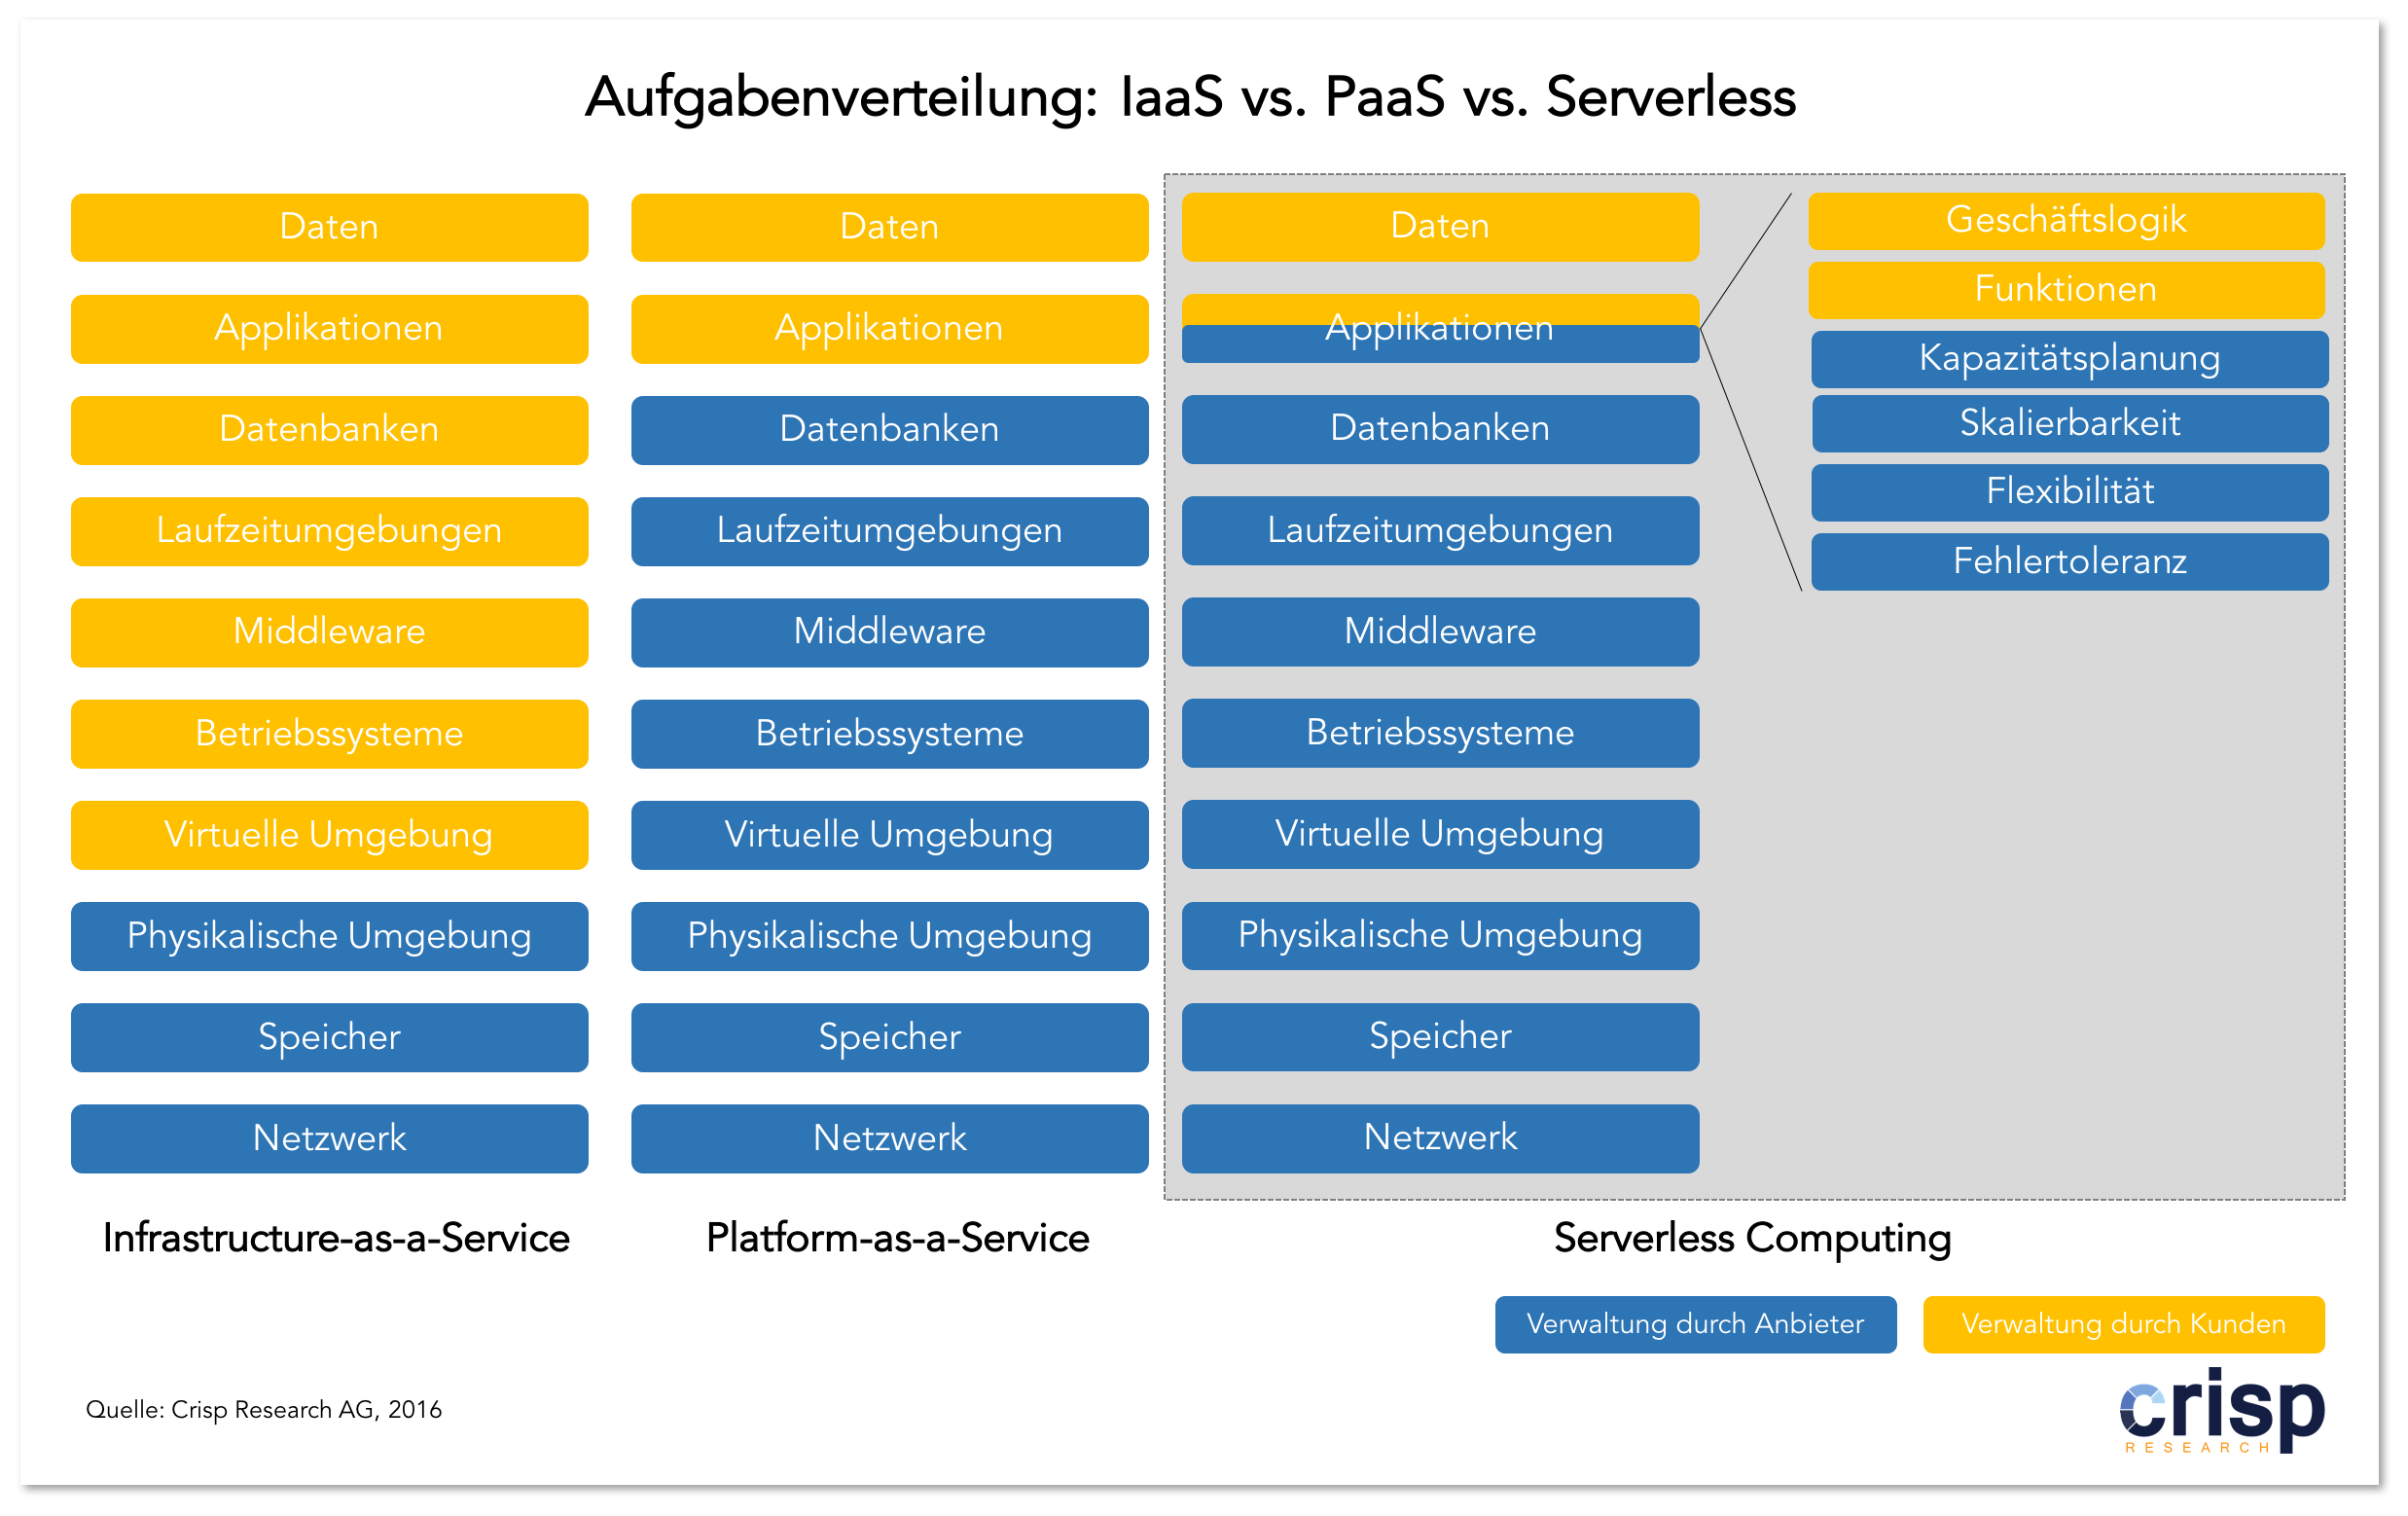
\includegraphics[scale=0.36]{./pics/IaaS_vs_PaaS_vs_Serverless.eps}
%\end{wrapfigure}
\section{SaaS} 
\label{sec:saas}
\newacronym{SaaS}{SaaS}{Software as a Service}
\acrfull{SaaS} kann als ein Service beschrieben werden, der OS-Images mit konfigurierbaren Diensten wie Datenbanken, Webanwendungen usw. bereitstellt. \acrshort{SaaS} gestaltet sich benutzerfreundlich, da die Konfiguration und das Deployment dieser Softwaredienste nicht erlernt werden müssen, um sie in eine größere Anwendung einzubinden. Anfallende Gebühren berechnen sich nach der Nutzungsdauer.
Viele traditionelle Software bietet seine \acrshort{SaaS} nicht an. Dies Impliziert laut Chandrasekaran, K. dass dieses Serviceliefermodell sich für Anwendungen nicht gut eignet wegen folgenden Punkten:
\newacronym{SLA}{SLA}{Service Level Agreement}
\begin{itemize}
	\item Geringe Latenz kann durch die Entfernung der gespeicherten Daten für Echtzeitanwendungen nicht gewährleistet werden.
	\item Die Datensicherheit kann nicht sichergestellt werden, da die mitbeteiligten Drittanbieter bei \acrshort{SaaS} die \acrfull{SLA} von Kunden nicht immer erfüllen.
	\item Anforderungen bestimmter Software verlangen eine Zentralisierung und eine Lokalisierung vor Ort, anders als bei \acrshort{SaaS}. 
\end{itemize}

\newglossaryentry{virtualization}{name={Virtualisation},description={Abstraktion der Anwendung, OS oder DB von der darunterliegende Infrastruktur z.B. ein Server.}}

%Diese Softwaredienste lassen sich zwar aggregieren, aber die Skalierung des daraus resultierende Softwarestacks erfolgt durch Notifikation des Drittanbieters, wodurch  

%Das \glqq\Gls{virtualization}\grqq\ einer ganzen Umgebung oder Stack zerteilt sich in eine Sammlung von kleinen spezialisierten Aufgaben, die durch Drittanbieter implementiert wurden. Dieser Fakt steigerte die wirtschaftlichen Kosten und machte die Skalierungsmöglichkeiten komplexer\cite{patternAWS}.


\chapter{FaaS}%{nichtfunktionalen/technischen Anforderungen zur Entwicklung des Serverless-Ansatzes}

\acrfull{FaaS}\label{sec:faas} kann als ein Rechenservice beschrieben werden, der nach Anfrage isoliert, unabhängig und granular ausgeführt wird. Komplexe Probleme wie horizontale und vertikale Skalierbarkeit, Fehlertoleranz und Elascitity werden von Kunden nur noch nach Bedarf konfiguriert und von dem Anbieter verwaltet. Die Besonderheit von \acrshort{FaaS} ist die \glqq Unit of Deployment\grqq\ und die Skalierung in Form einer Funktion. \cite{patternAWS}

Events\label{par:event-reaction} innerhalb eines verteilten Systems müssen verwaltet werden. Technologien wie Virtualisierte oder Containerized Server erzeugen neue Serverinstanzen zur Verarbeitung von einer Kette von variablen Events, die danach gelöscht wird.\cite{lambdaAWS} Die entstehende Problematik ergab sich durch eine starke Zunahme an Elementen, die einen hohen Verwaltungsaufwand forderten.  Was zurück auf die oben genannten Aufgaben \ref{sec:iaas-aufgaben} führte.

Polling\label{par:polling} ist der Ausdruck für eine zyklische Abfrage über einen Status z.B. von Ports oder Locks über Ressourcen. Die Verwendung von Systemressourcen ist ineffizient im Vergleich zu Alternativansätzen wie z.B in dem Push- oder Pull- Kommunikationsmodell.\cite{lambdaAWS} 

Funktionale Programmierung ist ein Programmierparadigma, in dem Funktionen nicht nur definiert und angewendet werden können, sondern auch wie Daten miteinander verknüpft, als Parameter verwendet und als Funktionsergebnisse auftreten können. Zustand und mutable Daten werden vermieden damit Seiteneffekten nicht entstehen und die Komposition flexibler wird. Das stellt einen Vorteil für die Skalierung eines Softwarekomponenten dar.\cite{funcScala}


Die Implementierung einer solchen Funktion geschieht durch die Auswahl der Programmiersprache und der von dem Cloud-Anbieter vorgegebenen Funktionsfassade. Diese wird vom Cloud-Anbieter aufgerufen, stellt aber keine zusätzlichen Bibliotheken bereit, daher ist es nötig, dass die auszuführende Datei alle Abhängigkeiten enthält.


Der Fokus bei \acrshort{FaaS} liegt auf der Quellcodeentwicklung und nicht auf dem Provisioning von Servern, der Installation von Software, dem Deployment von Containern oder auf konkreten Details der Infrastruktur.

%HTTP, Funktionale Programmierung, Fassaden, ... ?? 
%Funktionale programmierung abstrahiert. auf Infrastruktur. ??? 

Für die Betrachtung, ob \acrshort{FaaS} eine Lösung für eine konkrete Problemstellung ist, folgt eine Auflistung von Kriterien:
\paragraph{Es ist nicht empfehlenswert \acrshort{FaaS} zu benutzen, wenn:}
\begin{itemize}
	\item der Entwickler Rootzugriffsrechte auf alle Ressourcen eines Servers benötigt.
	\item die Priorisierung von Betriebssystemattributen wie CPU, GPU, Networking oder Speichergeschwindigkeit angefordert ist.
	\item Sicherheit relevant ist. Unautorisierte Zugriffe können mit \acrshort{FaaS} nur auf Systemebene erkannt werden.
	\item dauerhafte Prozesse angefordert sind.
\end{itemize}
\paragraph{Es ist empfehlenswert \acrshort{FaaS} zu benutzen, wenn:}
\begin{itemize}
	\item Aufgaben als Reaktion auf Events erledigt werden. 
	\item ein Scriptbehälter für z.B Cron Aufgaben benötigt wird. Die Zugriffsrechte sind beschränkter, Fehler sind einfacher zu erkennen und an einer Stelle aggregiert ( siehe CloudWatch ), des weiteren können Deployments einfacher angestoßen werden.
	\item die Skalierung des Servers bei einer ressourcenintensiven Verarbeitung vermieden werden soll.\ref{sec:pipes-filters}
	\item Services vorgegeben sind, die selten benutzt werden.
	\item die Verwaltung von \acrshort{API}-Server umgangen werden soll.
\end{itemize}\cite{lambdaAWS}


\chapter{Serverless-Angebote und Architekturen}

\paragraph{Die Softwarearchitekturen} helfen uns zu kommunizieren, welchen Zweck unsere Software erreichen möchte. Ihre \textbf{Entwurfsmuster} bieten generische Lösungen für wiederkehrende Probleme bei der Softwareentwicklung.


Auf konventionelle Webanwendungen wird hier Bezug genommen, als ein System, das über Presentation-, Data-, and Logik-Tiers verfügt. Jedes Tier kann mehrere Logik-Layers enthalten, die für unterschiedliche Funktionalitäten der Domains verantwortlich sind. Logging ist ein Beispiel für Cross-Cutting Concern, das Layers überspannt. Die Komplexität der Anwendung wächst zusammen mit der Beschichtung.
Eine Überprüfung der Architektur ist sinnvoll, wenn eine erfolgreiche Codeänderung von einer Anderen abhängt.

\newacronym{SOA}{SOA}{Service Oriented Architecture}
\paragraph{\acrfull{SOA}}
\label{sec:soa} unterlegt der Annahme, dass ein System aus mehreren kleinen, austauschbaren, wiederverwendbaren und entkoppelten Diensten besteht. Für die Entwicklung und Integration solcher Systeme bietet \acrshort{SOA} eine Menge von Entwurfsprinzipien und Standards. Entwickler stellen autonome Services her, die durch Nachrichtenübergabe kommunizieren und oft einen Schema haben oder eine Schnittstelle, die definiert wie die Nachrichten erzeugt werden.\cite{cloudEssentials}

\begin{figure}[H]
	\centering	
	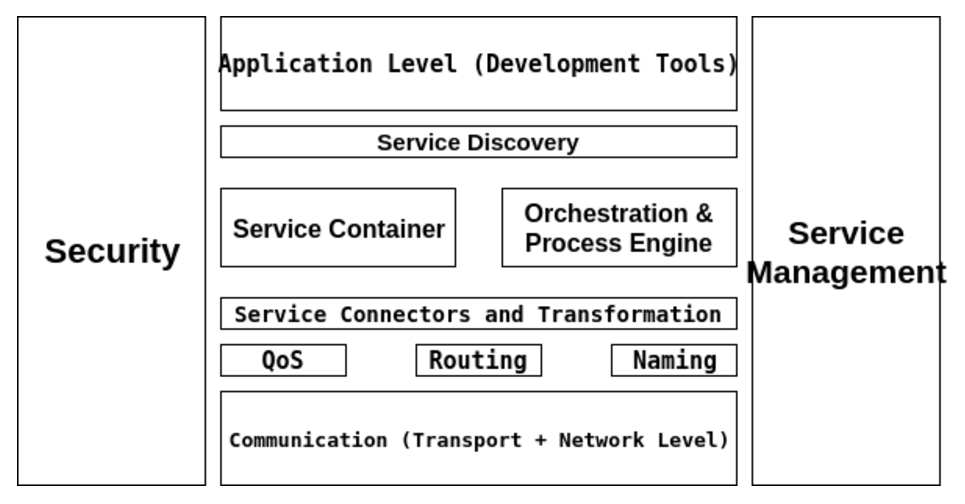
\includegraphics[scale=0.80]{./pics/arch-soa.eps}
	\caption{SOA Architekturreferenz\cite{archSoa}}
	\label{pic:arch-soa}
\end{figure}


SOA ermöglicht gegenseitigen Datenaustausch zwischen Programmen von unterschiedlichen Anbietern, ohne dass zusätzliche Änderungen an den Services vorzunehmen sind. Die Bestandteile eines solchen Architekturstils sind sowohl Standardschnittstellen als auch voneinander unabhängige Services\cite{archSoa}. 

Der Fokus in der Cloud liegt daher auf Service und Servicekomposition \cite{cloudEssentials}.

\newacronym{DSL}{DSL}{Domain Specific Language}
Microservices und Serverless versuchen die Komplexität der SOA ( \autoref{pic:arch-soa} ) anzusprechen. Beide Ansätze führen  Separation of Concerns, häufige Deployments und Heterogene \acrfull{DSL} mit sich.\cite{microAdv}

Auf einer Seite können Microservices ihren Zustand und Daten speichern und mit Hilfe von Frameworks implementiert werden. Auf der anderen Seite sind Serverless zustandlos, ihre Datenspeicherung ist zeitlich begrenzt und sie unterstützen Frameworks nicht direkt. ConnectWise\cite{ConnectWise}, Netflix\cite{Netflix} und UNLESS\cite{UNLESS} sind Beispiele für Unternehmen, die auch von Serverless Architekturen profitieren.


\newacronym{EDA}{EDA}{Event Driven Architecture}
\textit{\acrfull{EDA}} ist eine Softwarearchitektur, in der das Zusammenspiel der Komponenten durch Ereignisse gesteuert wird. Die Ereignisorientierung besitzt das Potenzial, dass die Architekturen von Anwendungen agiler, reaktionsschneller und
echtzeitfähig werden. Laut Ralf Bruns und Jürgen Dunkel ist \acrshort{EDA} für komplexe Fachlogik, große Datenvolumina, geringe Latenzzeit, Skalierbarkeit und Agilität geeignet.\cite{archEDA}\\
Die Serverless Technologien können durch Benachrichtigungen gestartet werden. Dieser \acrshort{EDA}-Stil verstärkt die Entkopplung auf einer temporären Ebene zwischen Producer und Consumer. Weiterhin ermöglicht ein Kommunikationskanal zur Benachrichtigung eine asynchrone Verarbeitung, ohne dass das System auf Grund von Fehlern abstürzt. \cite{patternIntegrationEnterprise}

Zusammenfassend sind folgende Vorteile ersichtlich:
\begin{itemize}
	\item Die Wiederverwendung von Services in unterschiedlichen Anwendungen senkt die Entwicklungskosten und den Time-To-Market.
	\item Durch die Standarisierung der Services kann ein System mit einer Rekonfiguration und ohne Weiterentwicklung schnell  auf die geschäftliche oder externe Bedürfnisse angepasst werden. Somit wird ein agiles Arbeiten möglich.
	\item Das Monitoring hilft Fehler zu erkennen und die Leistung zu messen.
	\item Aggregate von bereitgestellten Services können komplexere und domainübergreifende Aufgaben ausführen.
\end{itemize}\cite{cloudEssentials}

\newacronym{REST}{REST}{REpresentational State Transfer}
Im späteren Kapitel wird REST als Teil des \acrshort{EDA}-Architekturstils vorgestellt.


\section{Serverless}
\label{sec:serverless}

\newacronym{API}{API}{Application Interface}
Serverless kann als ein Ansatz beschrieben werden, der die Verwendung von einem Rechenservice, Dienste von Drittanbietern, von \acrfull{API}s und die Anwendung von Architekturmustern fördert. Ein solcher Anwendungsfall ist die Kommunikation mithilfe eines \glqq Delegation-Tokens\grqq\ zwischen den Front- und Back-End Diensten. \acrshort{FaaS} ist nur ein Aspekt dessen.


Serverless übernimmt die Entwurfsprinzipien von \acrshort{SOA} und \acrshort{EDA} \ref{sec:soa} und daher ergeben sich laut Sbarski folgende Richtlinien:
\newacronym{SRP}{SRP}{Single Responsability Principle}
\begin{itemize}\label{par:serverless-principles}
	\item Ein Rechenservice wird genutzt, um  Quellcode auf Anfrage auszuführen, kein Server.
	\item Zustandslose Funktionen unterliegen dem \acrshort{SRP} Prinzip.
	\item Für den Architekturentwurf werden Push basierte ereignisorientierte Pipelines genutzt.
	\item Front-Ends werden durch die Einbettung von mehr Zuständigkeiten verstärkt.
	\item Dienste von Drittanbieter dem Schreiben von eigenem Quellcode bevorzugt.
\end{itemize}\cite{serverlessArchAWS}

Die Vernetzung von zustandslosen Funktionen erlaubt, komplexe Systeme zu entwerfen, die einfach zu skalieren sind.
\newacronym{MVC}{MVC}{Model View Controller}
Die Komplexität und längerfristige Wartbarkeit des Systems lässt sich dadurch reduzieren, dass der Controller und/oder Router aus dem \acrfull{MVC} \cite{fowlerBlogMVC} vom Back- zum Front-End verschoben wird und Dienste von Drittanbieter hinzugefügt werden. \cite{patternAWS}


\begin{wrapfigure}{l}{0.36\textwidth}
	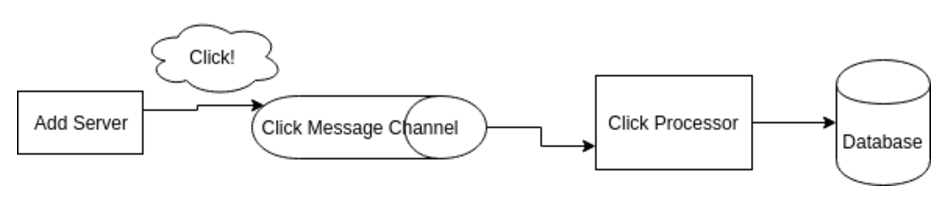
\includegraphics[scale=0.30]{./pics/classic-example.eps}
	\caption{Classic Add Server}
	\label{pic:classic-add}
\end{wrapfigure}

In einem beispielhaften konventionellen AdServer wird nach einem Click auf eine Werbung eine Nachricht über ein Kanal an einen Clickprozessor geschickt, der innerhalb einer Anwendung ausgeführt wird.\\ \\ \\

\begin{wrapfigure}{l}{0.36\textwidth}
	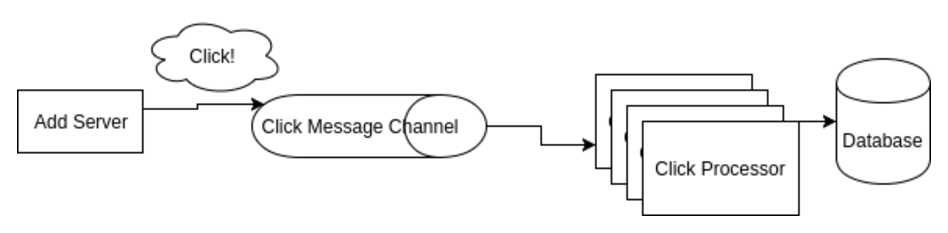
\includegraphics[scale=0.30]{./pics/serverless-example.eps}
	\caption{Serverless Add Server}
	\label{pic:serverless-add}
\end{wrapfigure}

Mit dem Serverless Ansatz wird dieser Clickprozessor pro Nachricht als eine neue Instanz der Funktion ausgeführt. Ihre Laufzeitumgebung und ihr Messagebroker wird von dem Cloudanbieter verwaltet. \cite{fowlerBlogServerless}\\
 

Dazu wird für den Entwurf von Serverless Architekturen eine Reihe von Mustern von unterschiedlichen Autoren vorgeschlagen.\\


\subsection{Pipes and Filters, Compute as a Glue}
\label{sec:pipes-filters}
\begin{wrapfigure}{l}{0.36\textwidth}
	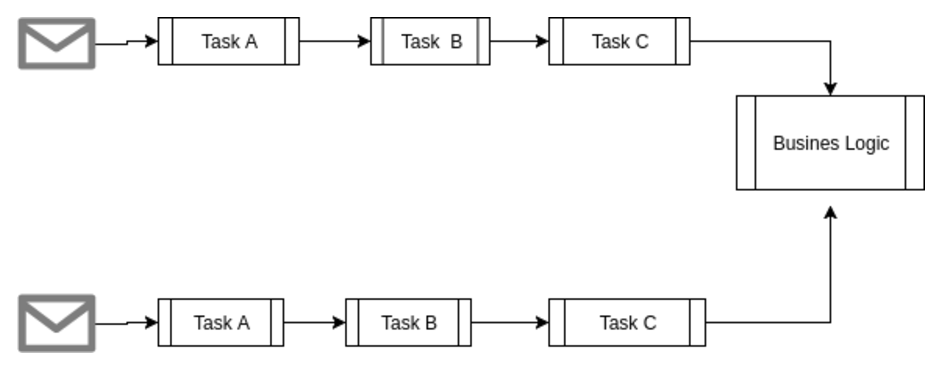
\includegraphics[width=0.9\linewidth]{./pics/pipes-and-filters.eps}
\end{wrapfigure}
Eine Anwendung kann Aufgaben von unterschiedlicher Komplexität ausführen. In einem monolithischen Modul sind das Refactoring, die Optimierung und die Wiederverwendung erschwert. \\
Zunächst werden die Aufgaben in diskrete Elemente ( oder Filter ) nach dem \acrshort{SRP} zerteilt und in einer Pipeline kombiniert. Dies hilft redundanten Quellcode zu vermeiden, ihn zu löschen, zu ersetzen oder zu integrieren in zusätzliche Komponenten, sich sobald die Aufgabenanforderungen ändern\cite{patternsCloud}. Ein weiterer Vorteil besteht darin, dass ein Flaschenhalseffekt vermieden wird, in dem mehreren Instanzen erzeugt werden, falls ein Element nicht genug Ressourcen für die Verarbeitung hat. 


\subsection{Legacy Api Proxy}
\begin{wrapfigure}{l}{0.36\textwidth}
	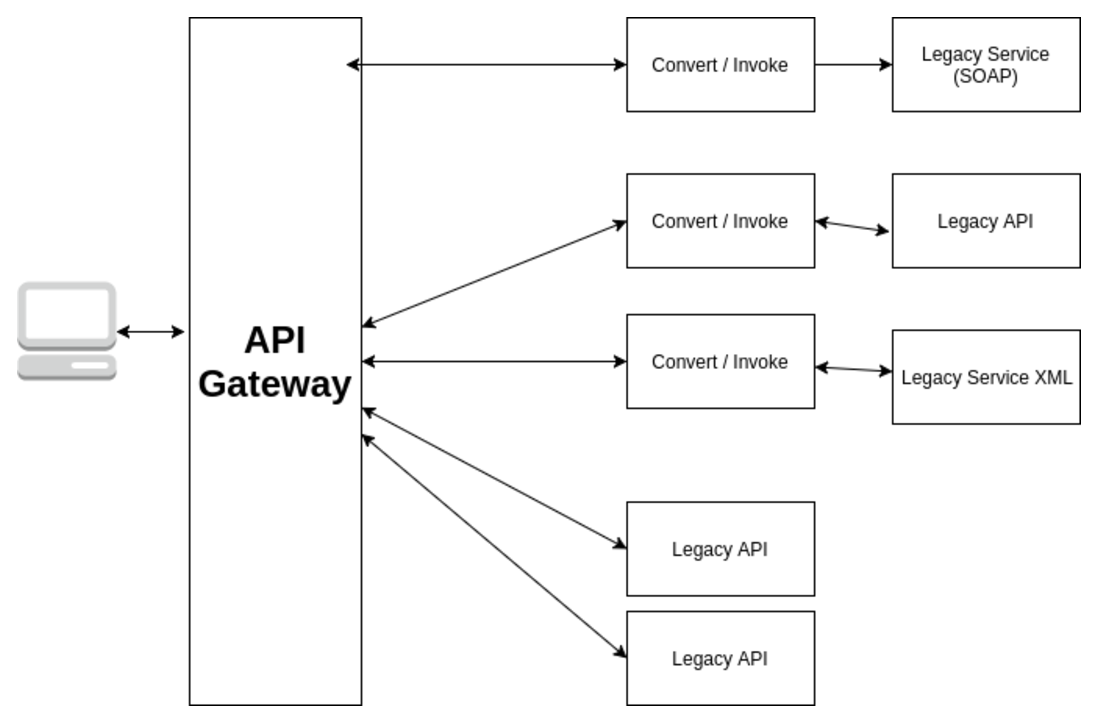
\includegraphics[width=0.9\linewidth]{./pics/legacy-api-proxy.eps}
\end{wrapfigure}
Wenn eine \acrshort{API} veraltet oder schwer zu benutzen ist, kann eine extra ( RESTful ) \acrshort{API} in den Vordergrund gestellt werden, die in gesonderten Prozessen Daten transponieren und für die angeforderten Formate aufstellen ( marshall ). Dies ist besonders nützlich, wenn die Legacy-Services selten benutzt werden. Zusätzlich erleichtert die Api Proxy die Integration mit anderen Architekturansätzen.
\\
\\


\subsection{Compute as a Backend}
\begin{wrapfigure}{l}{0.46\textwidth}
	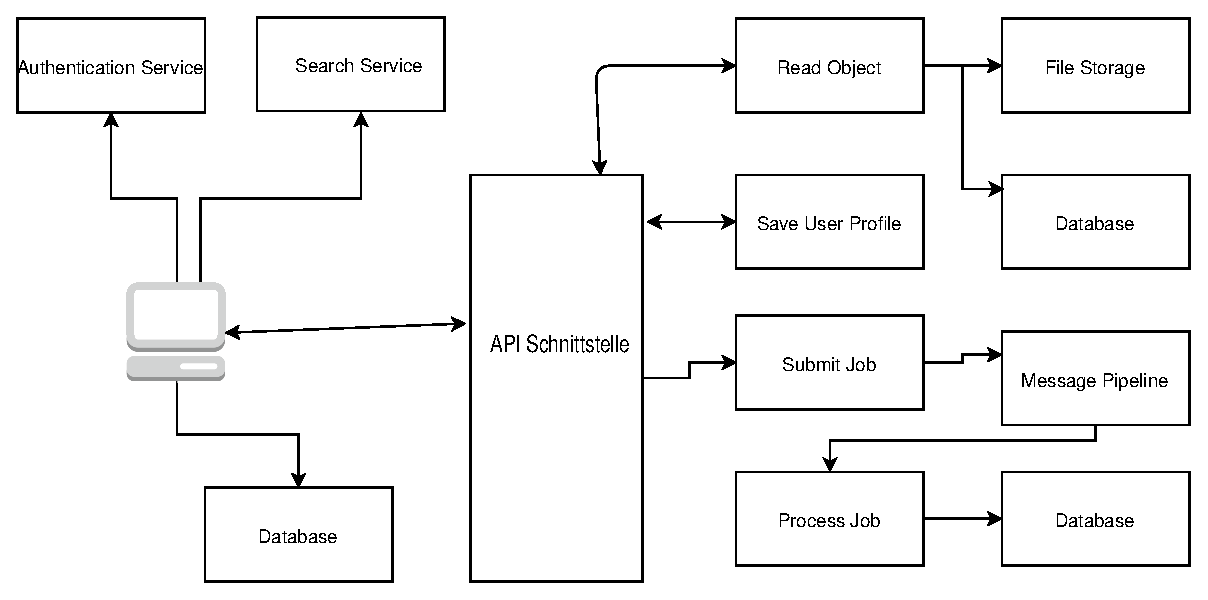
\includegraphics[scale=0.36]{./pics/compute-as-a-backend.eps}
	\caption{Compute as a Backend}
	\label{pic:compute-backend}
\end{wrapfigure}
Obwohl der Client direkt mit Services kommunizieren kann, müssen vertraute Informationen geschützt werden, indem sie das Back-End verarbeitet\cite{serverlessArchAWS}. Diese Aufgaben können hinter einer \acrshort{REST} Schnittstelle koordiniert werden. Wie in \autoref{par:serverless-principles} erwähnt, minimieren die Einbettung der Dienste von Drittanbietern und verstärkte Front-Ends den Fußabdruck des eigenen Back-Ends.

\subsection{Graph Query}
\begin{wrapfigure}{l}{0.36\textwidth}
	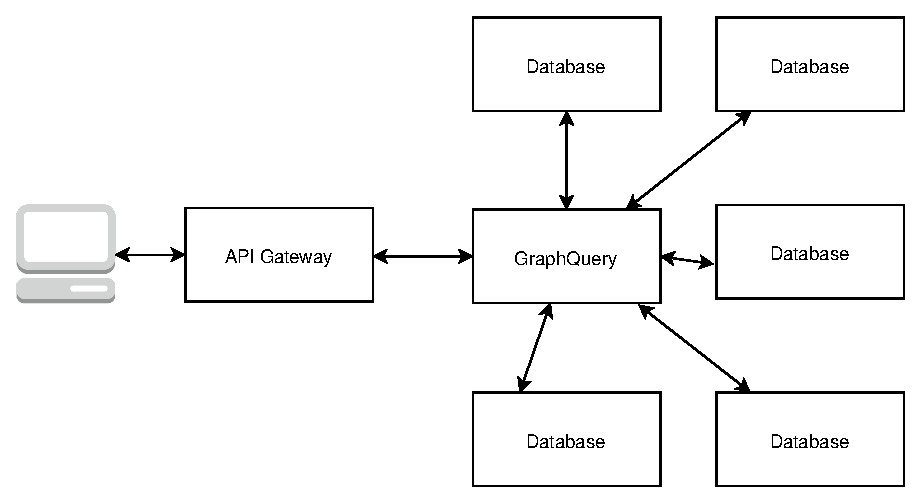
\includegraphics[scale=0.36]{./pics/GraphQuery.eps}
	\caption{Graph Query}
	\label{pic:graph-query}
\end{wrapfigure}
Wenn mit einer Anfrage mehrere Datenbanken abgefragt werden, entstehen multiple Paketumlaufzeiten ( Round-Trip ). Stellt eine \acrshort{REST} Schnittstelle in einer Anfrage zu wenig Queryparameter zur Verfügung, dann entsteht Overfetching, weil die Anfrage nicht präzise genug ist. Dagegen kann der Client die Parameter für die Abfrage spezifizieren und das Back-End baut sie zusammen und führt sie aus.


\subsection{Real time processing}
\begin{wrapfigure}{l}{0.36\textwidth}
	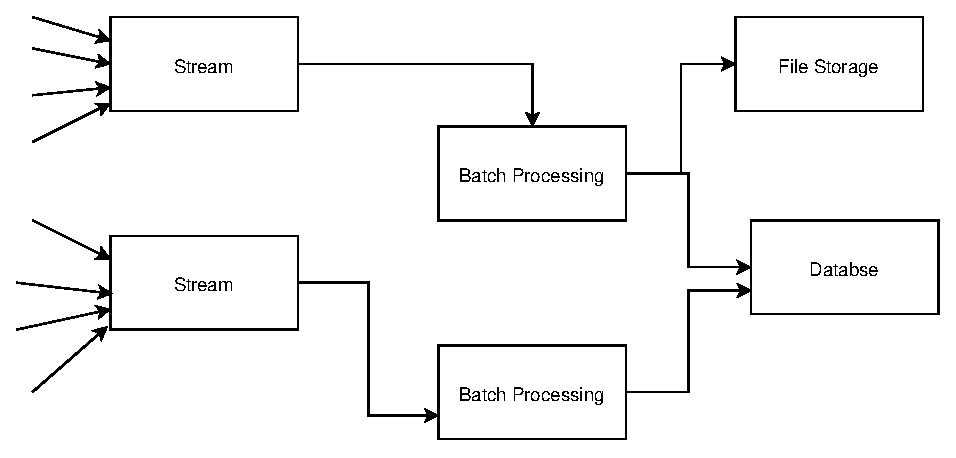
\includegraphics[scale=0.36]{./pics/real-time-processing.eps}
	\caption{Real Time Processing}
	\label{pic:real-time-processing}
\end{wrapfigure}
Die Verarbeitung von Streams in Echtzeit kann durch einen Buffer, der je nach Konfiguration die Daten weiter an den Worker leitet. Einen wesentlichen Vorteil stellt die unabhängige Skalierung des Streams und des Workers je nach Anfrage dar. Bei fehlerhafter Verarbeitung werden die Prozesse neu angestoßen.
\\
\\

%Competing consumers als pattern für die implementaiton vom Kommunikation kanal für events die lambdas triggern.

%Pipes and Filters\cite{patternsCloud} <-> lambda event driven
%Health endpoint monitoring <-> EC2 certificate
%Leader election -> TRansaction mngmt S3


%Queue Based Load Leveling -> Not appliable for Lambda Computing Model
%Retry ->
%Runtime Reconfiguration <-> Api Gateway Zero Downtime on Redploy
%Scheduler Agent supervisor -> Not needed if Design to Failure.
%Sharding -> Divide DataStore to Scale better -> Dynamo db + S3
%Static Content Hosting -> Solved by S3
%Throttling -> Scallability of Serverless Solved vs Transaction
%Vallet key <-> Auht0

\subsection{Priority Queue}\label{sec:priority-queue}
\begin{wrapfigure}{l}{0.36\textwidth}
	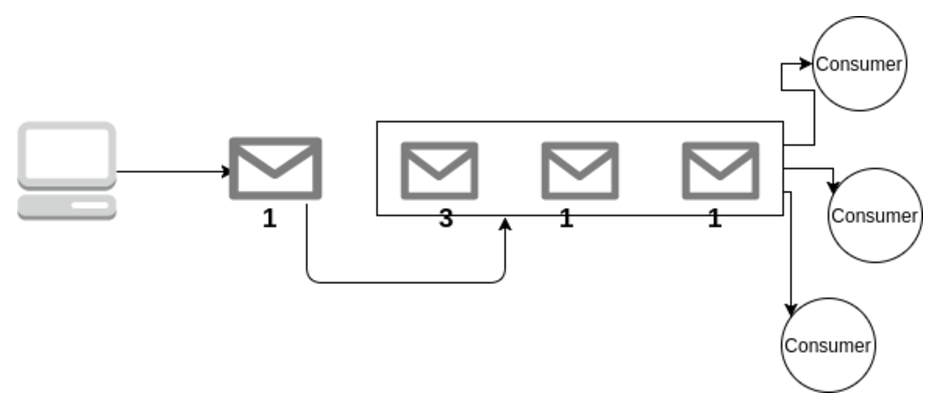
\includegraphics[scale=0.36]{./pics/pattern-priority-queue.eps}
	\caption{Priority Queue}
	\label{pic:priority-queue}
\end{wrapfigure}
Anwendungen können spezifische Aufgaben delegieren, wie z.B die Integration mit anderen Anwendungen und Services. Am Beispiel einer FIFO ( First In First Out ) Queue können die Nachrichten nach Priorität automatisch sortiert und asynchron verarbeitet werden. Für Systeme ohne integrierte Priorisierung können mehrere Queues für unterschiedliche Prioritäten benutzt werden und die Anzahl von Consumerprozessen wird entsprechend angepasst. Im letzteren Fall wird dabei die Starvation von Nachrichten, mit geringer Priorität, vermieden.

Das Priority Queue wird im Rahmen des Entwurfsmusters Competing Consumers als ein Consumerservice aufgefasst. Steigt stark die Anzahl an Anfragen die Kapazitäten des Systems, kommt zu seiner Überbelastung. Ein Consumerservice als Moderator von Anfragen ist im Stande das zu verhindern.



\subsection{Fan Out}
\label{sec:fan-out}
\begin{wrapfigure}{l}{0.45\textwidth}
	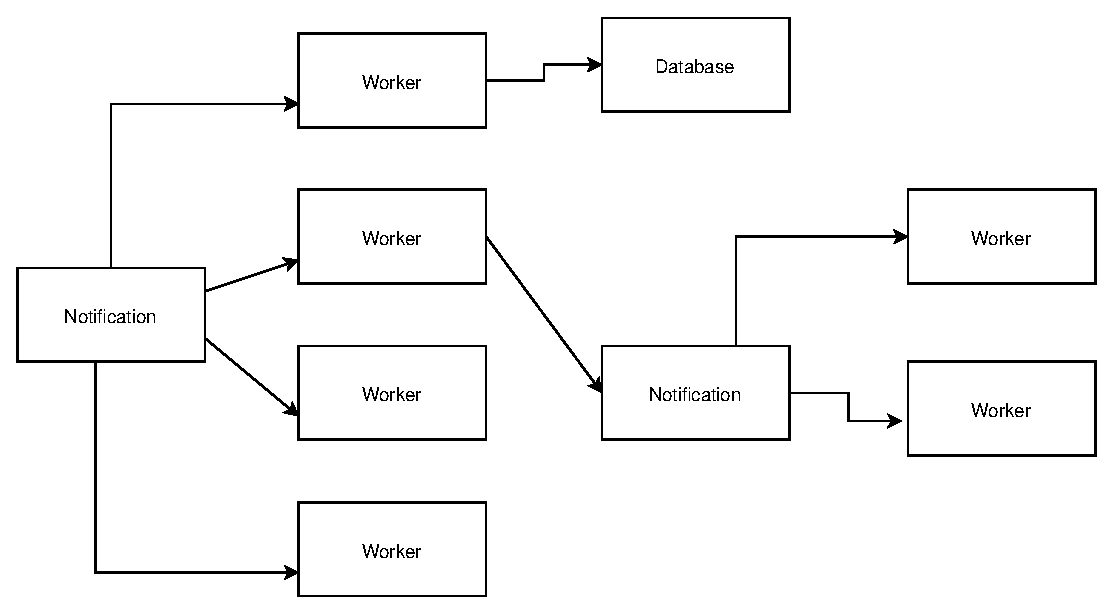
\includegraphics[height=3cm]{./pics/pattern-fan-out.eps}
	\caption{Fan Out}
	\label{pic:fan-out}
\end{wrapfigure}
Bei dem Eintritt eines Events können ein oder mehrere Subscriber durch die gepushte Benachrichtigung angestoßen werden. Damit wird ein Kommunikationskanal \ref{sec:priority-queue} zur Verwaltung von Nachrichten wiederverwendet und extra Geschäftslogik umgangen, z.B. kein Command Pattern für die gleiche Funktionalität\cite{serverlessArchAWS}.

\subsection{Federated Identity}\label{sec:federated-identity}
\begin{wrapfigure}{l}{0.36\textwidth}
	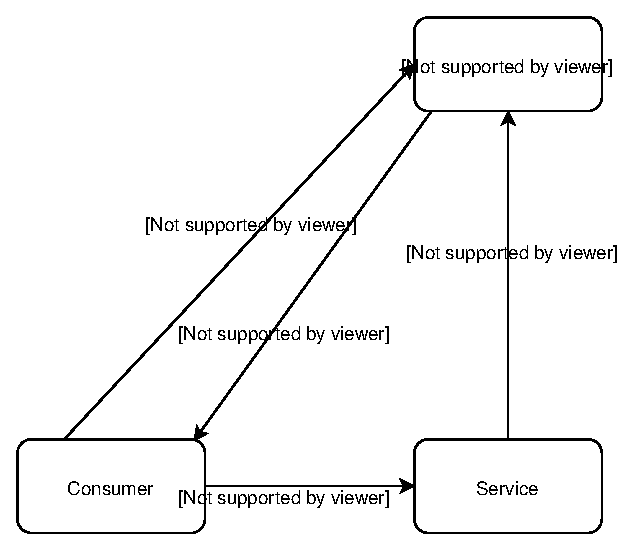
\includegraphics[scale=0.36]{./pics/pattern-federated-identity.eps}
	\caption{Federated Identity}
	\label{pic:federated-identity}
\end{wrapfigure}
Benutzer arbeiten mit multiplen Anwendungen von unterschiedlichen Organisationen. Um gleiche Zugangsdaten für Benutzter wiederverwenden zu können, wird dem Nutzer eine Identität bei einem Drittanbieter zugeteilt, diese wird mit einem Token an die Anwendung weitergeleitet. Der Authentisierungscode kann daher von dem Anwendungscode abgetrennt werden, damit kann zusätzliche Codierung für die Authentisierung vermieden werden .

\chapter{AWS-Serverless-Angebote}
\label{chap:aws-serverless}
\acrshort{AWS} ist ein Cloudandbieter
% Andere Anbieter 
% 3 sätze über AWS als Anbieter

\newacronym{JVM}{JVM}{Java Virtual Machine}
\begin{wrapfigure}{l}{0.16\textwidth}
	
\includegraphics[width=0.9\linewidth]{./pics/aws/Compute_GRAYSCALE_AWSLambda.eps}
\end{wrapfigure}
\paragraph{Lambda}\label{par:lambda} ist ein Rechenservice, der aus Quellcode und dessen Abhängigkeiten besteht. Die horizontale Skalierung erfolgt automatisch, elastisch und vom Cloudanbieter verwaltet; währenddessen die vertikale nach Konfiguration erfolgt. Lambda wird als Einheit für die Skalierung und das Deployment benutzt. \acrshort{AWS} unterstützt Javascript, Python, C\# und Java. Die letzte Programmiersprache betrifft das Konzept \glqq Cold- und Warm run\grqq\ besonders, da es nötig ist, die \acrfull{JVM} in ihrer Laufzeitumgebung hochzufahren ( cold run ). Der Cloudanbieter stützt sich auf das Pull- und Push- Kommunikationsmodell. Bei Pull überprüft die Lambda Laufzeitumgebung in regelmäßigen zeitlichen Abständen, ob Events z.B. bei Kinesis eingetreten sind und ruft die entsprechende Lambda Funktion mit einer Event-Datennutzlast auf. Bei Push ruft die Eventquelle z.B S3 je nach Konfiguration ( event source mapping ) die entprechende Lambda Funktion auf. 


\begin{wrapfigure}{l}{0.16\textwidth}
	
\includegraphics[width=0.9\linewidth]{./pics/aws/MobileServices_GRAYSCALE_AmazonAPIGateway.eps}
\end{wrapfigure}
\paragraph{API Gateway} ist eine Fassade, um Operationen sicher auszuführen, wie die Benachrichtigung von Kunden per Email und deren Identitätsüberprüfung. Weil AWS die Skalabilität von API Gateway und von Lambda übernimmt, ist die Bereitstellung und Wartung von EC2 Instanzen und die Konfiguration deren Load Balancer nicht mehr nötig. 

\begin{wrapfigure}{l}{0.16\textwidth}
	
\includegraphics[width=0.9\linewidth]{./pics/aws/Messaging_GRAYSCALE_AmazonSNS.eps}
\end{wrapfigure}
\newacronym{SNS}{SNS}{Simple Notification Service}
\paragraph{\acrfull{SNS}}\label{par:sns} erweitert das schon gut etablierte Beobachtermuster, in dem es einen Kanal für Events hinzufügt. Die konzeptionelle Technologie hinter \acrshort{SNS} wird \glqq Publish-Subscribe Channel\cite{patternIntegrationEnterprise}\grqq\ Muster genannt und entspricht den oben genannten \glqq Fan Out\grqq\ \ref{sec:fan-out} Architekturmustern. AWS kann durch Redundanz mindestens eine Lieferung der Nachricht gewährleisten.


\newacronym{S3}{S3}{Simple Storage Service}
\newacronym{SQS}{SQS}{Simple Queue Service}
\begin{wrapfigure}{l}{0.16\textwidth}
	
\includegraphics[width=0.9\linewidth]{./pics/aws/Storage_GRAYSCALE_AmazonS3.eps}
\end{wrapfigure}
\paragraph{\acrfull{S3}} ist ein Speicherdienst, der durch \acrshort{SNS} \ref{par:sns} die Events ( z.B das Löschen oder Erzeugen eines Objektes ) an \acrshort{SNS}\ref{par:sns}, \acrfull{SQS} \ref{par:sqs} oder Lambda schicken kann. \glqq Buckets\grqq\ sind Verzeichnisse auf der höchsten Ebene des Verzeichnissystems. Ein Objekt ist eine Kombination von Daten, Metadaten und eines Keys, der innerhalb des Buckets eindeutig ist.


\begin{wrapfigure}{l}{0.16\textwidth}
	
\includegraphics[width=0.9\linewidth]{./pics/aws/Database_GRAYSCALE_AmazonDynamoDB.eps}
\end{wrapfigure}
\paragraph{DynamoDB} ist eine NoSQL Datenbank. Ihre Tabellen bestehen aus Items ( Zeilen ) und deren Attributen ( Spalten ). Die Datenbank hat laut \acrshort{AWS} unendliche Datenkapazitäten und der Datenverkehr ist unbegrenzt. 
Durch automatische Skalierung mindert sich die Leistung nicht. Bei der Änderung eines Zeilenwertes in DynamoDB ist die Konfiguration eines Anstoßes der Lambdafunktion möglich.

\begin{wrapfigure}{l}{0.10\textwidth}
	
\includegraphics[width=0.9\linewidth]{./pics/aws/Messaging_GRAYSCALE_AmazonSQS.eps}
\end{wrapfigure}
\paragraph{\acrfull{SQS}}\label{par:sqs} ist eine message queue. Sie erlaubt die Interaktion von mehreren Publishers und Consumers in einer \acrshort{SQS} und automatisch den Lebenszyklus der Nachrichten verwaltet und kontrolliert Auszeiten ( Time out ) oder individuelle Verzögerungen.

\begin{wrapfigure}{l}{0.10\textwidth}
	
\includegraphics[width=0.9\linewidth]{./pics/aws/Analytics_GRAYSCALE_AmazonKinesis.eps}
\end{wrapfigure}
\paragraph{Kinesis Streams} ist ein Service für Echtzeitverarbeitung von Datenstreams. Es wird für Logging, Datenimport, Metriken, Analytics und Reporting benutzt. Ein Kinesis Stream ist eine sortierte Folge von Datensätzen, die auf \glqq Shards\grqq\ verteilt sind. Diese definieren die Kapazität des 'Durchsatzes' ( Throughtput ) von einem Stream und können nach Bedarf vergrößert werden.


\newacronym{RDS}{RDS}{Relational Database Service}
\begin{wrapfigure}{l}{0.10\textwidth}
	
\includegraphics[width=0.9\linewidth]{./pics/aws/Database_GRAYSCALE_AmazonRDS.eps}
\end{wrapfigure}
\paragraph{\acrfull{RDS}} hilft bei dem Setup und Wartung von mySQL, MariaDB, Oracle, MS-SQL, PostreSQL und Amazon Aurora mit automatischer Bereitstellung ( provisioning ), Sicherung, patching, recovery, repair und Fehlererkennung. \acrshort{RDS} kann durch \acrshort{SNS} \ref{par:sns} über eigene Events berichten.




\newacronym{SES}{SES}{Simple Email Service}
\begin{wrapfigure}{l}{0.10\textwidth}
	
\includegraphics[width=0.9\linewidth]{./pics/aws/Messaging_GRAYSCALE_AmazonSES.eps}
\end{wrapfigure}
\paragraph{\acrfull{SES}} behandelt die Absendung und die Empfangsoperationen wie Spamfilterung, Virus Scann und Ablehnung nicht vertrauter Quellen. Emails können weiterhin in \acrshort{S3} gespeichert, an Lambda versendet oder eine \acrshort{SNS} Benachrichtigung erstellen.

\chapter{KOMA, eine Beispielanwendung}\label{sec:KOMA} 
Im Folgenden wird eine Beispielanwendung, unter Verwendung der in \autoref{chap:aws-serverless} genannten Entwurfsmuster, implementiert.
\newacronym{EQF}{EQF}{European Qualifications Framework}

Die Beschleunigung der Veränderungen in der heutigen Gesellschaft und der technologischen Landschaft prägt sich in Bildung und Beruf in so fern aus, dass die heutigen Rahmenlehrpläne nicht mehr fachlich, sondern an der Kompetenzentwicklung orientiert sind, um u.a Kompetenzprofile für Lerner zu erstellen. Es existiert bereits ein anerkannter Europäischer Rahmen\cite{EQF} für Kompetenzbildung: \acrfull{EQF}. Am Beispiel von Sachsen-Anhalt\cite{BildungsServerSachsen} werden diese Kompetenzorientierung auf die spezifischen Bedürfnisse der Schule beschrieben und die Unterrichsstunden entsprechend gestaltet.

Die Anwendung soll für die pädagogische Diagnostik und Intervention genutzt werden.
Ziel der Umsetzung ist es daher, auf einer Seite die von einem Schüler erworbenen und zu erwerbenden Kompetenzen und deren Niveau nachzuvollziehen. Andererseits bietet sie das Potenzial die Bildungs-, Unterrichts- und Stundenplanung zu unterstützen.\\

Kommt diese Anwendung in Bildungsinstitutionen zum Einsatz, dienen die Rahmenlehrpläne als Leitpfad für die Bezeichnungen und Anforderungen der Kompetenzen, wohingegen \acrshort{KOMA} für die Organisation der einzelnen Fachrichtungen oder Lehrveranstaltungen zuständig ist. Da der \acrshort{EQF} als Basis mit internationaler Anerkennung genutzt wird, den Kompetenzstand eines Individuums abzubilden, wird die Bildungsqualität international vergleichbar.

Den Kern von \acrshort{KOMA} bildet die Zuweisung von Aktivitäten auf vordefinierte Kompetenzen. Erstere lassen sich einzeln oder in einer Sequenz anordnen. Sequenzen werden in Lehrveranstaltungen zusammengestellt. So können Aktivitäten, Sequenzen und Kompetenzen als Gestaltungsmittel für Lehrveranstaltungen genutzt werden. 
%Die Auswertung der Ergebnisse der Schüler erfolgt durch eine Entit

%Das Modell verfügt von eine Figur um die erledigte Aktivitäten auszuwerten, nämlich Evaluation.

Das folgende Beispiel beschreibt einen fachorientierten Ansatz zur Gestaltung von Lehrveranstaltungen:\\
Das Fach \glqq Web Computing \grqq\ lässt sich mit einer Sequenz von Lernaktivitäten ( Unterrichtseinheiten ) gestalten. Die zu behandelnden Themen erfordern grundlegendes Wissen und Fertigkeiten wie das Beschreiben von Kommunikationsprotokollen und Bash Scripting. Dabei ist zu beachten, dass Wissen und Fertigkeiten kumulativ wachsen und damit aufeinander aufbauen.

Im Gegensatz zu dem fachorientierten Ansatz wird nun der kompetenzorientierten Ansatz erläutert:
Das Kompetenzmodell differenziert unterschiedliche Kompetenzen in vielfältigen Zusammensetzungen. Ihre Fertigkeiten und/oder Wissen werden während der  Lernaktivitäten, bei der die Auswahl von Themen freigestellt ist, erworben.Durch die Sequenzierung von Lernaktivitäten baut sich das Kompetenzmodell aus.


\subsection{Anforderungsanalyse}
Die Auflistung \ref{list:koma-requirements} stellt einen für diese Arbeit angepassten Ausschnitt der Anforderungen für \acrshort{KOMA} dar:

\begin{itemize}\label{list:koma-requirements}
	\item Mit dem \acrshort{EQF} vergleichbare Kompetenzdefinitionen
	\item Berücksichtigen zukünftiger Erweiterungen 
	\item Abrufbarkeit durch den Browser 
	\item Private Datenspeicherung u.d Login
	\item Ertragen von großen Nutzlastschwankungen
\end{itemize}

\subsection{ER-Modell} Aus der Beschreibung von \acrshort{KOMA} \autoref{sec:KOMA} ergibt sich folgendes Modell.\autoref{list:koma-requirements}
\begin{figure}[h]
	\centering
	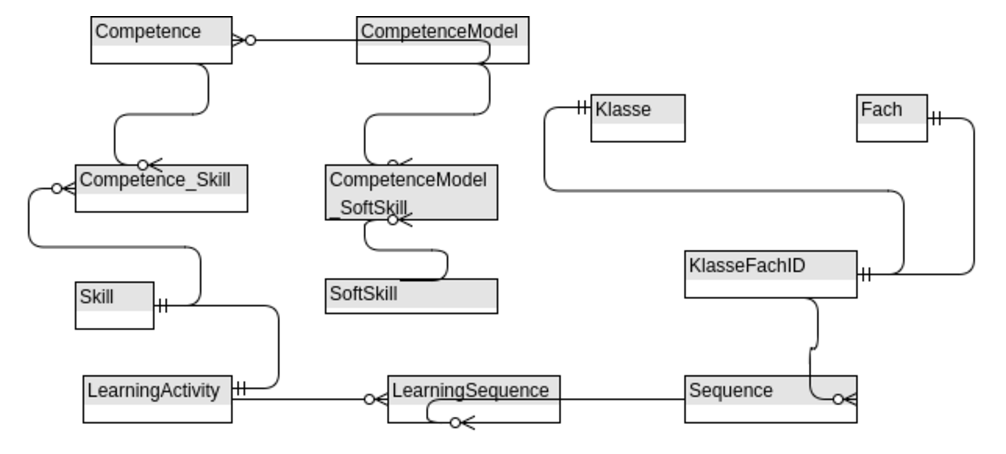
\includegraphics[scale=1]{./pics/koma-er-concept.eps}
	\label{pic:koma-er-concept}
	\caption{Entity-Relationship Modell für KOMA}
\end{figure}

Dieses ER-Diagramm \autoref{list:koma-requirements} definiert die Beziehungen zwischen den in \autoref{sec:KOMA} beschriebenen Konzepten. Eine Kompetenz ( Competence ) besteht aus Fertigkeiten ( Skill ), die in einer Lernaktivität ( LearningActivity ) erworben werden. Die Letztere gehört zu einer Sequenz von Lernaktivitäten ( LearningSequence ). Erworbene Kompetenzen können nach Klassenstufen und Fächern aufgerufen werden, damit ein Kompetenzstand abgeleitet werden kann. Das Modell ermöglicht die Gestaltung von \acrshort{EQF}-konformen Kompetenzprofilen ( CompetenceModel ).



\subsection{Komponentenübersicht}
\label{sec:components}

Um einen Anhaltspunkt zu geben, werden hier die Softwarekomponenten beschrieben.

Bei dem Aufruf der Website im Browser präsentiert sich ein \glqq Sign in\grqq\ Knopf zum Einloggen und verschiedene Möglichkeiten zur Formulierung einer Abfrage. Diese ist in einem \acrshort{S3} Bucket als statische Webseite gelagert.
Wird der Knopf zum Einloggen gedrückt, fordert eine Weiterleitung ( mit dem dargestellten Schlüssel ) die Authentisierung des Benutzers an. Mit der erfolgreichen Operation kehrt die Nutzeransicht mit einem \glqq Token\grqq\ auf die Webseite zurück. Der erhaltene Token wird als Autorisierung-Parameter in dem \glqq HTTP Request Header\grqq\ mit den nächsten Anfragen an das Back-End geschickt.

\newacronym{URL}{URL}{Universal Resource Locator}
Nach dem Login kann der Browser durch Absenden der nächsten Anfragen seinen Token zur Überprüfung übergeben. Die \acrshort{API} Gateway empfängt die Anfragen und transponiert deren Parameter, um zunächst die entsprechende Lambdafunktion synchron aufzurufen. Da die \acrshort{API} nach \acrshort{REST} entworfen ist, werden die Lambdafunktionen nach der \acrshort{HTTP}-Methode und der \acrshort{URL} abgebildet.

Dieser Loginprozess entspricht dem in \autoref{sec:federated-identity} beschrieben Federated Identity Muster.

Eine Anfrage an die \lstinline|GET https://<host>/page/{individual}| \acrshort{URL} führt die Lambdafunktion \glqq OWL Parser\grqq\ aus. Die Funktion liest die Datenbasis von S3 \glqq OWL Storage \grqq\ und extrahiert den Wert des \lstinline|{individual}|-Parameters, um eine Antwort zu generieren. Diese abstrahierte Zuweisung von \acrshort{URL}s auf Back-End Dienste entspricht einem \acrshort{REST} Ansatz. Dagegen erwartet die \lstinline|POST https://<host>/sparql| \acrshort{URL} eine Abfrage im \glqq Request Body\grqq\ der Anfrage mit dem Key \glqq Query\grqq\ , um sie auf der oben genannten Datenbasis auszuführen. Dabei unterstützt die Java Bibliothek Jena ARQ\cite{jenaARQ}


\begin{figure}[H]
	\begin{center}
		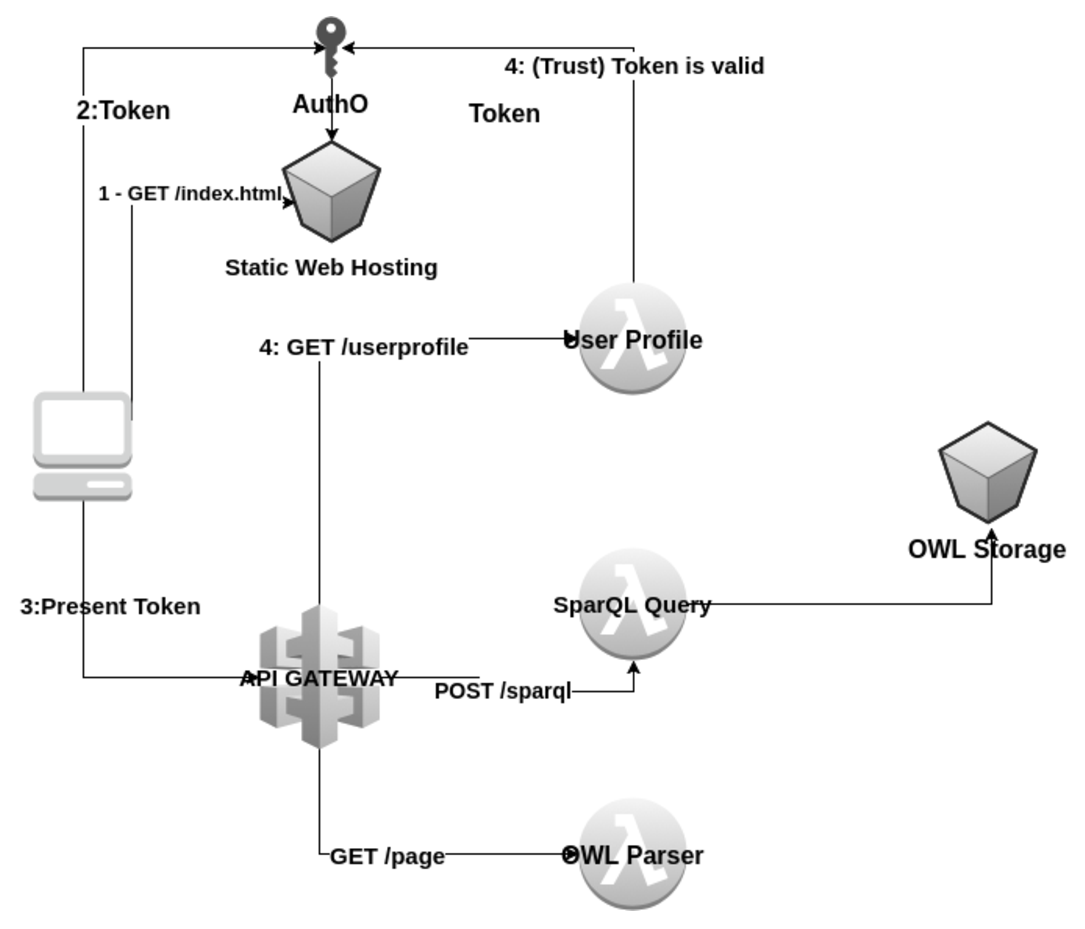
\includegraphics[scale=0.60]{./pics/static-web-hosting.eps}
		\caption{KOMA Components}
		\label{pic:koma-components}
	\end{center}
\end{figure}

\section{Umsetzung}
\label{chap:impl}
Die grundlegende Vorgehensweise bei der Umsetzung dieser Webanwendung gliedert sich zunächst in die Datenspeicherung und deren Analyse bzw. Auswahl. Als Zweites wird zwischen dem Entwurf mit den oben vorgestellten Serverless Architekturmustern und Technologien und deren Implementierung iteriert, um ein schnelles Feedback zu erhalten.

\subsection{Datenspeicherung- Analyse und Auswahl}
Die Gestaltung von Kompetenzmodellen und deren zukünftige Weiterentwicklung hängt stark von den spezifischen Bedürfnissen der jeweiligen Schulen ab. Die möglichen Erweiterungen oder Anpassungen des Modells stellt die Benutzung des einer relationalen Datenbank für \acrshort{KOMA} in Frage. In der folgender Tabelle werden die Eigenschaften von relationalen mit ontologischen Schemas verglichen.

%@Pre-Dev--> Tabelle 
\begin{table}[h]
	\caption{Vergleich relationalem mit ontologischem \ref{subsec:ontology} Schema}
	\centering{}
	\begin{tabular}{ccc}
		\noalign{\vskip\doublerulesep}
		Eigenschaft & Relational & Ontologisch \tabularnewline[\doublerulesep]
		\hline\noalign{\vskip\doublerulesep}
		Weltannahme & Existiert nur & Existiert mindestens \tabularnewline[\doublerulesep]
		\noalign{\vskip\doublerulesep}
		Individual & muss Unique & kann >= 1 \tabularnewline[\doublerulesep]
		\noalign{\vskip\doublerulesep}
		Info & Ableitung = x & ja \tabularnewline[\doublerulesep]
		\noalign{\vskip\doublerulesep}
		Oritentation & Data & Bedeutung \tabularnewline[\doublerulesep]
		
	\end{tabular}
\end{table}

Das ausgewählte Datendarstellungsformat ist das ontologische Schema, da es den Fokus auf Erweiterbarkeit und semantische Konzepte legt.
Im \glqq Semantic Web\grqq\ profitieren \glqq Linked Data Driven Web Applications\grqq\ von den vernetzten Datenbanken.
\cite{W3C}


\newacronym{W3C}{W3C}{World Wide Web Consortium}
Das \glqq Semantic Web\grqq ist eine Erweiterung des herkömmlichen Web, in der Informationen mit eindeutigen Bedeutungen versehen werden\cite{ontoWhat2}. Das \acrfull{W3C} spezifiziert eine Zusammenstellung von Standards und best practices für die Mitteilung von Daten und deren semantischer Darstellung.\cite{sparqlLearn}.
\newacronym{OWL}{OWL}{Web Ontology Language}
Diese Bedeutungen werden für Maschinen durch Ontologien dargestellt, welche in \glqq .owl \grqq\ Dateien gespeichert werden.\cite{W3C}

%\begin{figure}[h]
%	\centering
%	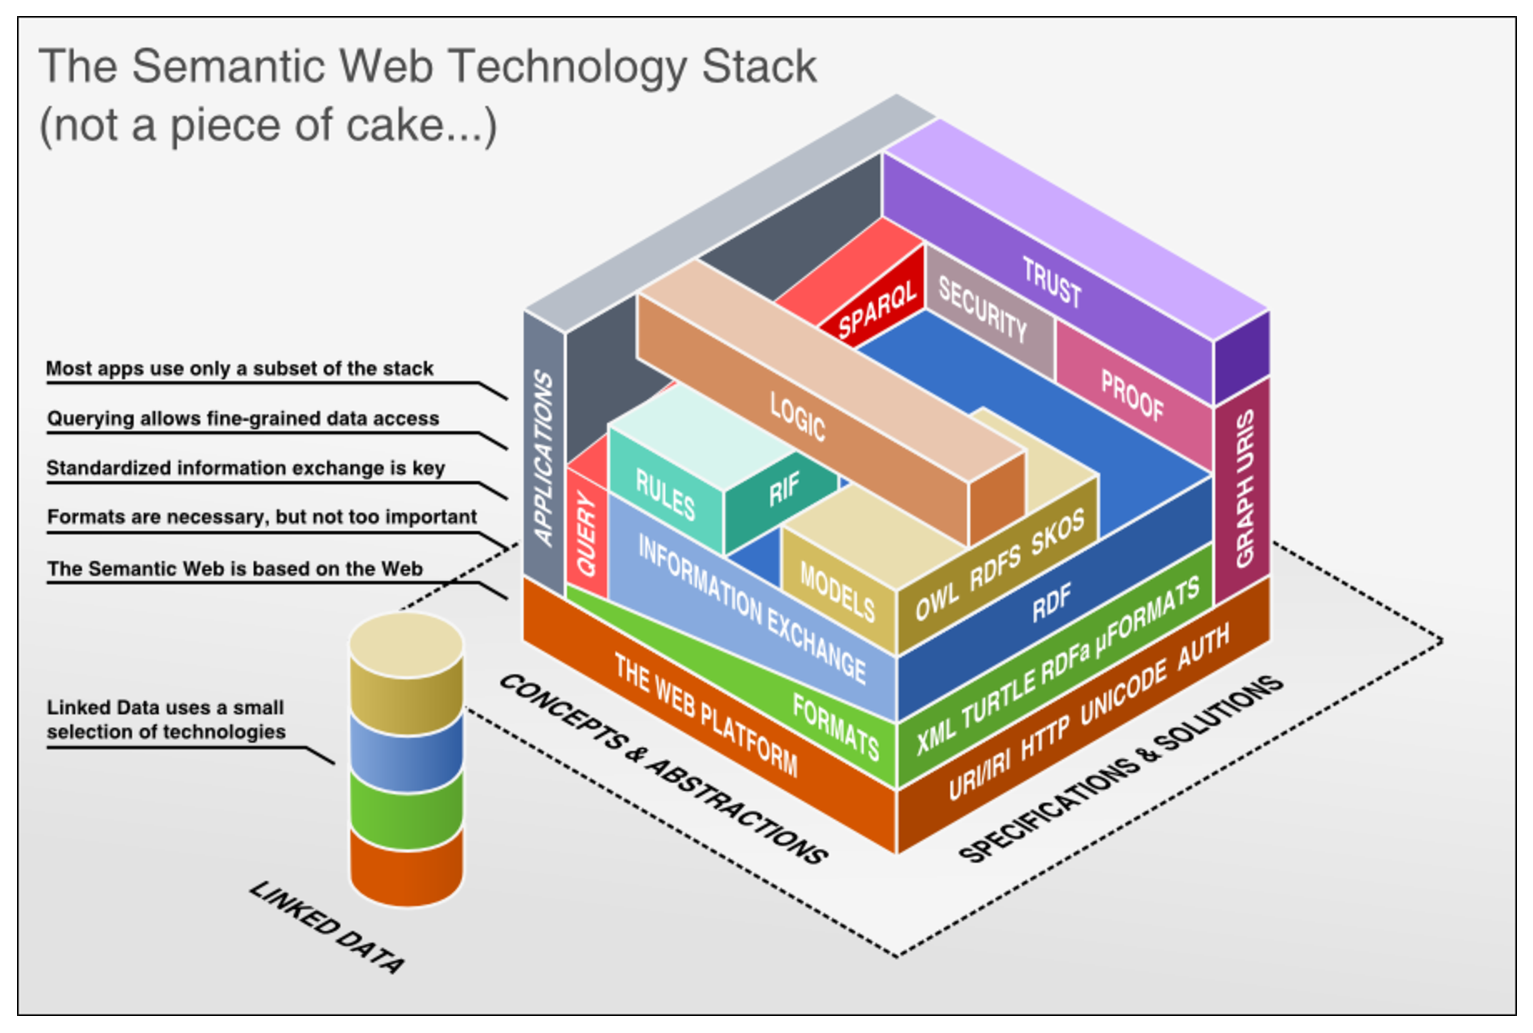
\includegraphics[width=0.8\textwidth]{pics/semantic_web_technology_stack.eps}
%	\caption{Überblick von Semantic Web Stack}
%	\label{fig:semantic-web-stack}
%\end{figure}


%@Def
Eine Ontologie\label{subsec:ontology} ist eine formale Spezifikation über eine Konzeptualisierung \cite{ontoWhat}. Die Denotation der dargestellten Signifikanten lässt sich durch ihre weltweit eindeutigen Präfix identifizieren z.B: \lstinline|PREFIX owl: <http://www.w3.org/2002/07/owl#>|  \cite{W3C}. Deren Beziehungen können zu externen Ontologie-signifikanten verweisen und dadurch ein Consensus über Begrifflichkeiten erreichen. 


Der Entwurf der Ontologie wurde nach Ontology-Engineering-101 durchgeführt:

Während der Umsetzung wurde Protégé \cite{Protégé} als unterstützende Anwendung benutzt.

Um bereits vorhandene Technologien zu nutzen,
wurde ein aktueller öffentlicher graphischer ontologischer Entwurf\cite{ontoMoodle} ( siehe \autoref{fig:competence-ontology} ), der in Moodle mit einer relationalen Datenbasis und PHP umgesetzt wurde, untersucht.

Eine Implementation dieser Ontologie ist jedoch nicht von Watson\cite{Watson} und LOD\cite{LOD} auffindbar.

\begin{figure}[h]
	\centering
	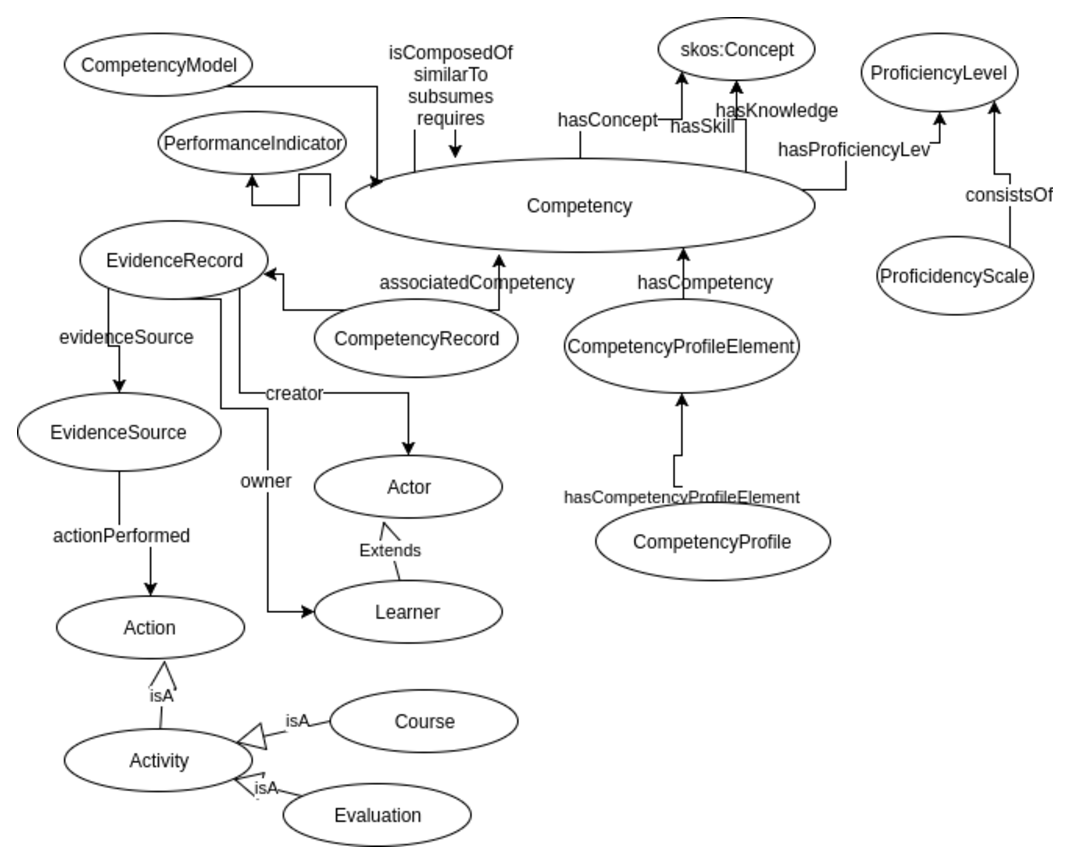
\includegraphics[angle=270]{pics/competency-ontology.eps}
	\caption{Kompetenzontologie}
	\label{fig:competence-ontology}
\end{figure}


Der Entwurf und seine Dokumentation lassen freie Interpretation über Begriffe und deren Zweck, z.B \glqq isComposedOf\grqq, \glqq subsumes\grqq. Ein Standard zur graphischen Darstellung ist zur Zeit noch nicht anerkannt. Graphische Benutzeroberflächen zur Darstellung und zum Entwurf von Ontologien sind derzeit entwickelt, z.B. Graphol \cite{graphol}.

\newacronym{RCD}{RCD}{Reusable Competency Definition}
Daher folgt eine beispielhafte Erklärung, die auf den Anwendungsfall \acrshort{KOMA} eine angepasste und ergänzende Interpretation der dargestellten Terminologie des Entwurfs und der \acrshort{RCD} ( s.u. ) liefert.

\begin{wrapfigure}{i}{0.36\textwidth}
	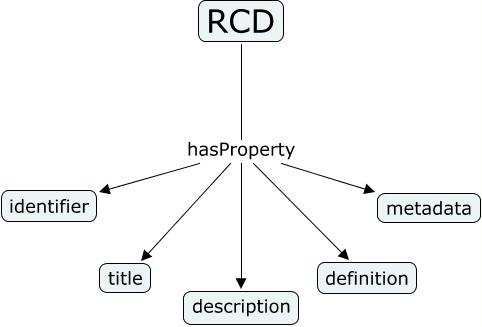
\includegraphics[width=0.9\linewidth]{pics/RCD.jpg}
	\caption{Reusable Competency Definition}
\end{wrapfigure}

Der \acrshort{EQF} wurde für die ontologische Darstellung beschrieben und bietet eine europäisch anerkannte Definition von Kompetenz, die \acrfull{RCD} \cite{eqfCompetency}. Diese ist jedoch nicht in einer veröffentlichen Datenbasis umgesetzt worden.


\newglossaryentry{Kompetenz}{name={Kompetenz},description={die bei Individuen verfügbaren oder durch sie erlernbaren kognitiven Fähigkeiten und Fertigkeiten, um bestimmte Probleme zu lösen, sowie die damit verbundenen motivationalen, volitionalen und sozialen Bereitschaften und Fähigkeiten, um die Problemlösungen in variablen Situationen erfolgreich und verantwortungsvoll nutzen zu können}}

Die zwei Leitmotive sind auf der einen Seite Kompetenzanforderungen, \glqq die festlegen, über welche Kompetenzen ein Schüler, eine Schülerin verfügen muss, wenn wichtige Ziele der Schule als erreicht gelten sollen. Systematisch geordnet werden diese Anforderungen in Kompetenzmodellen, die Aspekte, Abstufungen und Entwicklungsverläufe von Kompetenzen darstellen\grqq\ \cite{competence}. 

Auf der anderen Seite bildet die Definition von \Gls{Kompetenz} eine handlungsleitende Grundlage. Nach Weinert werden Kompetenzen als \glqq die bei Individuen verfügbaren oder durch sie erlernbaren kognitiven Fähigkeiten und Fertigkeiten, um bestimmte Probleme zu lösen, sowie die damit verbundenen motivationalen, volitionalen und sozialen Bereitschaften und Fähigkeiten, um die Problemlösungen in variablen Situationen erfolgreich und verantwortungsvoll nutzen zu können\grqq\ \cite{weinert2002leistungsmessungen}.

\newacronym{RDF}{RDF}{Resource Description Framework}
\newacronym{TURTLE}{TURTLE}{Terse RDF Triple Language}

Die bisher erreichte Analyse des Domainproblems wird nun anhand von Protégé in einen \acrfull{RDF} Format bzw. \acrfull{TURTLE} beschrieben. \acrshort{TURTLE} besteht aus einer für Menschen lesbaren Syntax und kann sowohl Ontologien in \acrshort{OWL} als auch \acrshort{Sparql} Abfragen darstellen. 

Das folgende \autoref{lst:turtle-triple} zeigt eine beispielhafte Darstellung von ontologischen Fakten, den sogenannten \glqq Triples\grqq\ . Diese bestehen aus Subjekt, Merkmal und Objekt. Die erste Zeile lässt sich wie folgt interpretieren: dem Namen einer fiktiven Schülerin Alice ( Subjekt ) wird ein Merkmal in Form einer Kompetenzausprägung ( Property ) innerhalb eines Unterrichtsfachs, das in Unterrichtsreihen oder -einheiten sequenziert werden kann, wie z.B Mathematik II ( Objekt ).

\begin{lstlisting}[language=SQL,caption={Darstellung von Triples in TURTLE},label={lst:turtle-triple}]
:Alice :hasCompetency :Math_II .
:EvidenceRecord rdf:type owl:Class .

:actionPerformed rdf:type owl:ObjectProperty ;
	rdfs:domain :EvidenceSource ;
	rdfs:range :Action .
\end{lstlisting}

\newacronym{Sparql}{Sparql}{Protocol And RDF Query Language}
Um aus Ontologien Informationen zu entnehmen, wird die Abfragesprache \acrfull{Sparql} 
verwendet. Diese ähnelt sich der traditioneller SQL. 

Die einfachste Abfrage in Sparql wählt alle Triples von dem abgefragten Datenmodell ( oder Graph ) wie in \autoref{lst:sparql-selectall} gezeigt wird.

\begin{lstlisting}[language=Sparql,caption={Sparql SELECT ALL},label={lst:sparql-selectall}]
SELECT * WHERE { ?s ?p ?o .}
\end{lstlisting}

Hilfsvariablen können deklariert werden, um Ergebnisse aus einem Triple als Parameter für das nächste zu benutzen. Die folgende Abfrage ließe sich \glqq Wähle alle Properties des Graphes und wähle alle dessen Subjekten mit Alice als Objekt\grqq formulieren. \\
\begin{lstlisting}
PREFIX owl: <http://www.w3.org/2002/07/owl#>
PREFIX rdf: <http://www.w3.org/1999/02/22-rdf-syntax-ns#>
PREFIX rdfs: <http://www.w3.org/2000/01/rdf-schema#>
PREFIX koma: <https://s3-us-west-2.amazonaws.com/ontology.thb.de/koma-complex.owl#>
SELECT ?x WHERE {
	?y rdf:type owl:ObjectProperty .
	?x ?y koma:Alice .
}
\end{lstlisting}

Wie in \autoref{sec:components} erwähnt wurde, Sparqlabfragen werden durch die \acrshort{API} Gateway für Lambda Transponiert.

%So dass auch die Benutzer von \acrshort{KOMA} solche Abfragen stellen können wird ein \glqq Sparql-endpoint\grqq mit Hilfe von Apache Jena ARQ, ein Sparql-Engine, zur Verfügung gestellt. 

%Dieser Sparql-Endpoint entspricht der Repositoryschicht der Anwendung und wird nach Anfrage von der Ontologie in S3 mittels Sparql JSON Objekte zurückliefern.
%Eine Lambdafunktion arbeitet als Schnittstelle \ref{lst:lambda-interface} zwischen die ARQ Bibliothek, den Client und die darunterliegende Infrastruktur.


\section{RESTful API}
\label{sec:rest}
\newacronym{HTTP}{HTTP}{Hypertext Transfer Protocol}
\newacronym{CRUD}{CRUD}{Create, Read, Update, Delete}
Der Entwurf von einer benutzerfreundliche \acrfull{HTTP} \acrshort{API} beinhaltet die Abstraktion von komplexe Geschäftslogik und Datenverarbeitung  in den vier \acrlong{CRUD} Operationen.

\newacronym{JSON}{JSON}{Javascript Object Notation}
Die Komplexität des darunterliegenden Datenmodells erlaubt eine \acrshort{REST} Schnittstelle nur einfache Abfragen zu formulieren.\cite{microAdv} Daher stellt \acrshort{KOMA} zusätzlich einen Sparql-Endpunkt für Komplexe Sparql Abfragen zur Verfügung. Die letzte Zeile der Tabelle \autoref{tab:rest} entspricht dem Letzteren.

\begin{table}[H]
	\caption{RESTful API}\label{tab:rest}
	\noindent 
	\centering{}
	\begin{tabular}{ccc}
		\hline
		\noalign{\vskip\doublerulesep}
		Methode & URL & Rückgabe\tabularnewline[\doublerulesep]
		\hline
		\noalign{\vskip\doublerulesep}
		GET & /ontology & Information über KOMA
		\tabularnewline[\doublerulesep]\noalign{\vskip\doublerulesep}
		\noalign{\vskip\doublerulesep}
		GET & /ontology/\{individual\} & RDF von Individual
		\tabularnewline[\doublerulesep]\noalign{\vskip\doublerulesep}
		GET & /page & Auflistung von Entitäten 
		\tabularnewline[\doublerulesep]\noalign{\vskip\doublerulesep}
		GET & /page/\{individual\} & Information über diesen Fakt
		\tabularnewline[\doublerulesep]\noalign{\vskip\doublerulesep}
		POST & /sparql & Abfragenergebnis
		
	\end{tabular}
\end{table}

AWS API Gateway ermöglicht die Definition, Konfiguration und das Importieren von Schnittstellen. Beispielsweise kann der Anfrageparameter in \lstinline|GET https://<host>/page/Alice}| mittels dem Muster in \autoref{lst:map-template} an dem Key \glqq individual \grqq\ zugewiesen werden. Hier handelt sich um einen \glqq body mapping template \grqq\ für den Inhaltstyp ( content type ) \glqq application/json\grqq\ .

\begin{lstlisting}[language=Javascript,caption={API Gateway Request Mapping Template},label={lst:map-template}]
https://<host>/page/{individua}
...
{
"individual" : "$input.params('individual')"
}
\end{lstlisting}

Nachdem eine Anfrage eingetreten ist und deren Parameter transponiert sind, erfolgt ein synchroner Aufruf der zuständigen Lambdafunktion. Die Verwaltung dieser Instanziierung entspricht den Priority Queue Muster in \autoref{sec:priority-queue}, wobei die \acrshort{API} Gateway die Queue und die Lambdafunktion die Consumers entspricht.
% Hier vtl. messaging channels ansprechen a- synch

Der folgende \autoref{lst:js-handler} zeigt die Implementierung einer Lambdafunktionsfassade, die für die oben genannte \acrshort{URL} zuständig ist. 

\begin{lstlisting}[language=Javascript,caption={Lambda Javascript Funktionsfassade},label={lst:js-handler}]
...
exports.handler = function (event, context, callback) {
	reqIndividual = event.individual; // check possible exception
	async.waterfall([createBucketParams
						, getS3ObjectBody
						, parseOntology
					],
					function (err, result) {
						if (err) {
							callback(res.createErrorResponse(500, err));
						} else {
						if (Object.keys(result).length === 0 && result.constructor === Object) {
							callback(null, res.createErrorResponse(404, "there was no result on the search"));
						} else {
							callback(null, res.createSuccessResponse(result));
...
\end{lstlisting}

Die zweite Zeile entspricht der Fassadensignatur von Lambda für Javascript. Das erste Parameter, \glqq event\grqq, enthält in dem Fall Informationen über die Ursprüngliche Anfrage. Das Zweite, \glqq context\grqq\, erlaubt den Zugang auf die Laufzeitumgebung von Lambda und kann definieren, ob die Ausführung erfolgreich ( \lstinline|context.success(Object result)| ), fehlerhaft ( \lstinline|context.fail(Error error)| ) oder als Kombination des zwei letzteren fertig  ( \lstinline|context.done(Error error, Object result)| ). 

In der Zeilennummer 4 befindet sich der Aufruf \lstinline|async.waterfall(...)|. Dieser entsprecht dem Waterfall Muster wessen Verarbeitungsschritte in der \autoref{pic:waterfall} dargestellt werden. 
Dieser Muster erlaubt eine Menge von Funktionen so zu verketten, dass das Ergebnis der Einer das Eingabeparameter der Nächsten ist. Wenn ein Fehler in eine Funktion entsteht, hält das Waterfall an. 

\begin{figure}[H]
	\begin{center}
	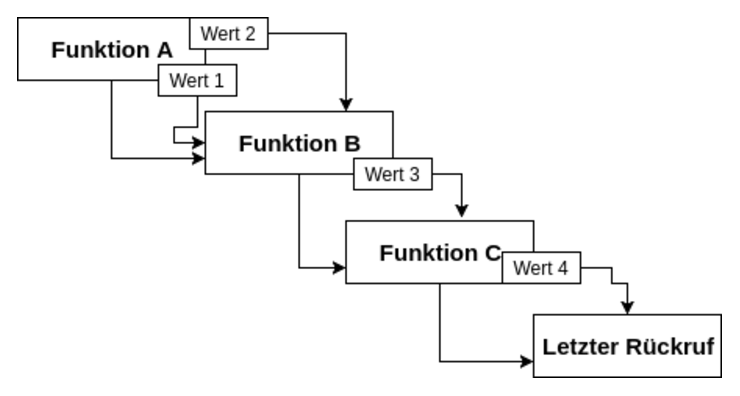
\includegraphics[scale=0.6]{./pics/aws/pattern-waterfall.eps}
	\caption{Waterfall Muster}
	\label{pic:waterfall}
	\end{center}
\end{figure}

Um die Wiederverwendbarkeit zu gewährleisten, ist die Abtrennung der  Abhängigkeiten in Bibliotheken von der Lambdafunktion sinnvoll. Dieser Ansatz wird von dem \acrshort{SOA}-Architekturstil \autoref{sec:soa} gefordert.



Im Fall von der \lstinline|POST https://<host>/sparql| \acrshort{URL} werden die Abfrageparameter wie in \autoref{lst:map-template-query} zum Key \glqq Query \grqq\ abgebildet.

\begin{lstlisting}[language=Javascript,caption={API Gateway Request Mapping Template Query},label={lst:map-template-query}]
{
"Query": "$input.params('query')"
}
\end{lstlisting}

Dieser erwartet die Abfrage in \acrshort{TURTLE} mit dem die im Body des HTTP-Requests in \acrfull{JSON} geschickt wird.


%Dieser Endpunkt unterstützt nicht nur GET-Abrufe, sondern auch POST-Anforderungen mit einer Nutzlast.Unter der verfügbaren SparQL endpoints Implementierungen

\paragraph{Regeln für Anfragen}
Der Zugang auf die Schnittstelle wird durch CORS konfiguriert um deren Ausnutzung zu vermeiden. 


%Um den Datenmodell möglichst simpel programmatisch abzufragen wird zunächst dessen Schnittstelle\ref{sec:rest} definiert. 

\subsection{Datenhaltung Synchronisierung und Replizieren}
\subparagraph{Master - Subordinate}
\begin{wrapfigure}{i}{0.10\textwidth}
	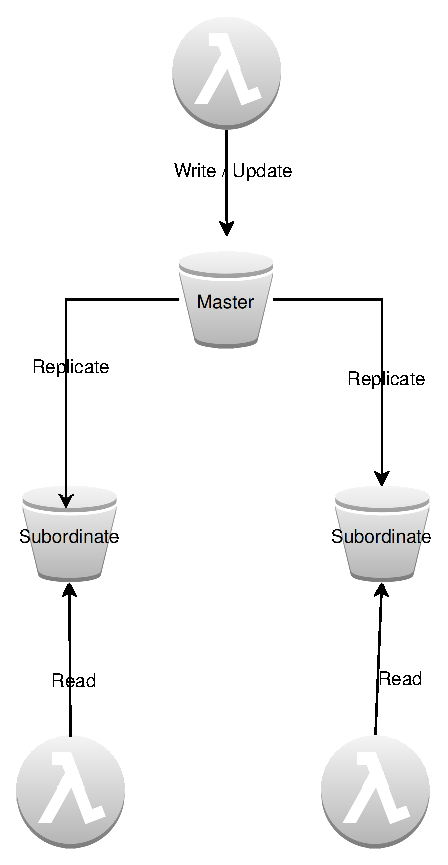
\includegraphics[scale=0.2]{./pics/aws/pattern-master-subordinate-data-replication.eps}
\end{wrapfigure}
Cloud Dienste werden oft in unterschiedlichen Datazentren oder Regionen deployed. Um die Verfügbarkeit, Performance und Konsistenz zu maximiereun und die Datenübertragungkosten zu minimieren, kann eine Master-Datenbasis mit erlaubte Read und Write Operationen und eine Subordinate-Datenbasis mit nur Read Operationen definiert werden. 
Der Master pusht oder ( one-way ) synchronisiert die Subordinate-Replikas. 
Diese Aufteilung favorisiert Read Operationen.


\subparagraph{cache shared }
\begin{wrapfigure}{i}{0.16\textwidth}
	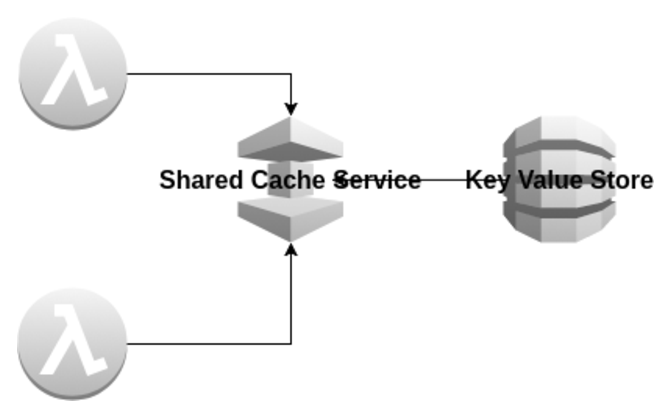
\includegraphics[scale=0.2]{./pics/aws/pattern-cache-shared.eps}
\end{wrapfigure}
Caching zielt auf die Verbesserung der Performance und Skalabilität eines Systems, in dem die oft gelesene Daten temporär zwischenspeichert werden. Es gibt zwei Typen von Cache: In-Memory und Shared-Cache. Die zustandslose Natur der Lambda kompliziert die Benutzung der ersten Cachevariante. 
Die Shared-Cache hilft das Problem zu beheben, bei Inkonsistenzen unter verteilten Caches. 


\subsection{Datenverarbeitung}

\subparagraph{Waterfall}
\begin{wrapfigure}{i}{0.16\textwidth}
	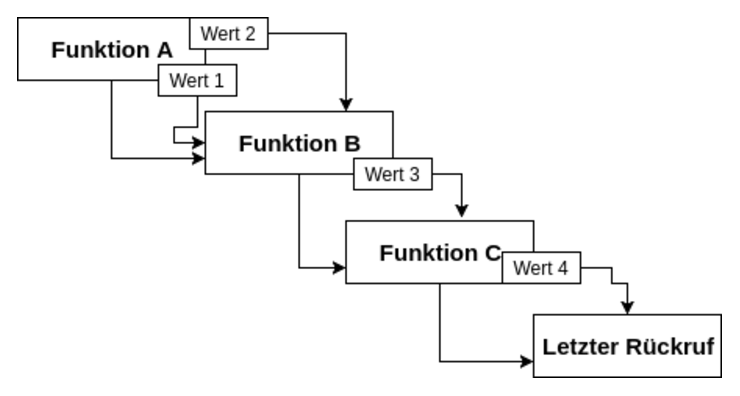
\includegraphics[scale=0.2]{./pics/aws/pattern-waterfall.eps}
\end{wrapfigure}
Dieser Muster erlaubt eine Menge von Funktionen so zu verketten, dass das Ergebnis der Einer als Eingabeparameter der Nächsten ist. Wenn ein Fehler in eine Funktion entsteht, hält das Waterfall an.


\subsection{Abtrennung des Monoliths}

Im Folgendem es wird beispielhaft eine abtrennung einer JEE Anwendung.

%\subparagraph{JEE.war} \glqq And\grqq Test vs SRP Identifizieren der Concerns und ihre Trennung: 

%\subparagraph{Einloggen} Login beispiel: user + password + userData -> user + passord -> uuID -> userData refactor and share common code


%Autorisierung und Authentifizierung. Einleitung

%Auth0 bietet Authentifizierung as a Service an. Der Benutzer erhält einen JSON Web Token JWT und schickt ihn Encoded JSON Web Signature JWS oder JSON Web Encription zur Anwendung mit.
%Mit wenige Konfigurationsschritte kann man die Benutzer Authentifizieren. 


%Einloggen: 0Auth Google gibt token, der wird in Lambda überprüft, Session in oauth.com verwaltet


%\subparagraph{Dynamo DB} Funtion: Read + Write + updateS3 zu Split S3, Split R/W 

%Datenspecherung Architektur:
%DynamoDB: speichert :individual als Schlussel und seine relative URL
%Ś3: speichert die .owl Dateien.

%Lambda Funktion: Maps zwischen S3 und DynamoDB.




\subsection{Single Page Application}
\label{sec:spa}

Da KOMA ohne Vorkenntnisse gebrauchsfertig sein soll, mit dem Fakt dass Milliarden von Desktop Geräte die Web mit einem Browser erkundigen können, lässt sich die Entscheidung über die Art der Benutzeroberfläche leicht Treffen.

Die Web Anwendung ist für alle Rechenaufgaben verantwortlich die im Browser aus dem Sicherheitssichtpunkt kein Gefahr darstellen, um den Backend oder Servers möglichst wenig auszulasten. Deswegen bietet sich eine Single Page Application an. 
Die SPA besteht aus ein einziges HTML Dokument. Dies vereinfacht man die Konfiguration der Authentifizierung und unterbricht den Fluss der UI-Darstellung zwischen Seiten.

Ein konfiguriertes Anfangsprojekt/Quickstart kann mithilfe von Initializr\cite{Initializr} oder JHipster\cite{Jhipster}. Für die lokale Entwicklung der Webseite werden anhand von NodeJS und NPM folgende Bibliotheken als Abhängigkeiten verwaltet: Bootstrap als Stylescheet und jQuery als Javascript-Bibliothek.
Die Webseite wird Statisch mittels S3 geliefert. Dies geschieht mit einem Befehl: 
\begin{lstlisting}[language=BASH, caption={Webseite veröffentlichen}]
$ aws  --region us-west-2 s3 website --index-document index.html --error-document error.html 's3://koma.thb.de'
\end{lstlisting} 

Da der Zugriff auf die Datenspeicherung gesichert werden soll, wird die Login-Funktionalität hinzugefügt.


\chapter{Bewertung}

\paragraph{Zur Skalabilität}
Skallabilität in Datenhaltung -> Entwerfe für Distribution + vorteile von Lokalität.
Read replikas -> evtl. Konsistent. 
Viele Perspektiven von Daten -> Lebenszyklus von Daten. 
---- Bounded Context ---- 
Service ist nicht nur Funktion oder nur DB.
Entkopplung fordert enkapsulation und Cohesion.

Event als Bussinesmanager -> Coordinator / Orchestrator -> Lambda
Als Finite State Machine oder WorkFlow

\paragraph{Anwendung}{Latenz}
Die entstandene Webanwendung befindet sich in US-WEST-2, Oregon, in den USA. 
Da keine Cache oder CDN Funktionalität weder Implementiert noch konfiguriert ist, ist die Latenz direkt proportional zur Ausführungsdauer der Lambda Funktion.
@Benchmark testing curl 
@Lambda Monitoring

In Zeiten des Cloud computings 
\paragraph{Frameworks und FaaS}
Frameworks helfen aber sind platform abhängig. Entweder JEE und JVM oder PHP.
Es kann auf die Layer of Abstraction in FW verzichtet werden. 
Die Ersetzbarkeit des FaaS entkoppelt die Anwendung und den Entwickler von der darunterliegende Technologie.

\paragraph{DevOps Frameworks}
Die benötigte Fertigkeiten für die Umsetzung einer Serverless Anwendung werden mithilfe von Deploymentframeworks gemindert. Die Aufnahme von 3.Anbieter ist deswegen notwendig. Es existieren bereits solche Hilfe wie z.B Serverlessframework@Ref

Risiko:
Entickler brauchen einen guten Testplan und eine gute DevOps Strategie.<- skills shortage

\paragraph{Transaktionen}
Transaktionen können nicht parallel ausgeführt werden. Sequenciel aka Messaging Pattern.
Zusammenspiel Arch. interfaces prog.modell und FW
Arch 1st -> def interfaces and interactions. to program to a inteface


Eventual consistency -> event driven + ontology quality
Consistenty -> koma-standalone <- transaction mgm

\paragraph{Vorteile}
Automatische Skalierung <!-- größe und kleine Apps --> und Fehlertoleranz
Automatisches Kapazitätsmanagement
Flexible Ressourcenverwaltung
Schnelle Bereitstellung der Ressourcen
Exakte nutzungsabhängige Abrechnung der Ressourcen
Konzentration auf den Kern des Source-Codes


\paragraph{Nachteile}


SLA Service Level Agreement: Latency, Bank:High volume Transactions,
Decentralisation of Services = Challenge = Overhead, time, energy <- orchestration of events.
Decentralisation vs monotithik != --komplexity
Kontrollverlust
Erhöhtes Lock-in Risiko

kurzlebige konfigurationen herausfinden ?? tracking?
viel Konfiguration, kaum Konveniton -> .json 4 everything
local testing braucht event-symulation.json



\paragraph{Zur Entwicklung}
Die Starke Komponentisierung und Dezentralisierung von Software, die Variabilität von Programmiermodellen, Frameworks, Tools, -Sprachen und dessen Entwicklungsumgebung erhöht die Komplexität des Enwicklungscyklus und hervorhebt die Bedürfnis von Tools zur Automatisierung von Tests, Deployment und Konfiguration. Also ein wohldefiniertes Handlungsplan bei der Softwareentwicklung dass von der nicht zu bearbeitende Details abstrahiert. 
Die DevOps Kultur spricht solche Probleme an. Neben dem Entwurf der Softwareachitekture  muss, um derer Umsetzung Zeitgemäß zu gewährleisten, eine zum Projekt passende DevOps Strategie.
Um Vorteil von der neuen Technologien zu nehmen, ist die Recherche nach schon existierenden DevOps Frameworks besonders wichtig. Dessen Integration in der DevOps Strategie diene für eine Agile Entwicklung.

\paragraph{Zum Datenmodel}
Aus der Anforderungs analyse einer Informations Techonologie Web Anwendung sind die Builder, Texste und dessen Darstellung das ergebniss, dass ohne Daten inhaltlos wäre. Auf eine Seite Das Relationale Datenschema stellt keine Semantik für sich dar, sondern durch von der Software entstandene Verknüpfung zwischen dem Endergebnis und dem Datenschema. Auf der Anderen Seite die  RDF Daten einer Ontologie \textit{is} das Modell.

\paragraph{Zum API Gateway}
Bei Frameworks wie JEE werden Schnittstellen zwischen Layers und Tiers bereitgestellt und diese am Laufzeit entdeckt aka Service Discovery. 
Im Fall der API Gateway wird die Kopplung bei derer Konfiguration festgelegt wo derer Rekonfiguration ein neues Deployment ohne Downtime bedeutet. Die Der Quellcode der Dienste bleiben unberührt und kein Load Balancer muss rekonfiguriert werden. 


\paragraph{Zum Serverless}
In dieser Arbeit wurde eine "nach buch" weise die Architektur gestalltet. Die unterschiedliche Interpretationen des Begriffs Serverless kann auch zu Kreativen anzätzen führen@AdamBien JEE
Es kann daher auch als Serverless betrachtet wenn neue Quelldataien eine Docker Instance neu Erzeugen oder nur Updaten, dessen LoadBalancing auch als Serverless Quellcode verpakt werden kann. 

\paragraph{Zur Annahme} dass Quellcode schneller entwickelt werden kann, wenn der Entwickler sich nur damit beschäftigt.

\chapter{Ausblick}



\paragraph{RESTful UI}
RESTful Anfragen für bestimmte UI formate.

\lstlistoflistings


\listoftables


\chapter*{Abkürzungen}
\markboth{Abkürzungen}{}


\begin{acronym}[Bash]


\acro{GC}{Garbage Collection}

\glqq Garbage Collection\grqq{} bezeichnet die automatische Speicherwaltung zur Minimierung des Speicherbedarfes eines Programmes.
\ac{GC} wird zur Laufzeit durch Identifikation von nicht mehr benötigten Speicherbereichen ausgeführt.
Im Vergleich zur manuellen Speicherverwaltung benötigt \ac{GC} mehr Ressourcen.

\end{acronym}

\bibliographystyle{alpha}
\bibliography{sources}


\end{document}



%@Glossar
%ontology: explicit, formal specification of a shared conceptualization
%Semantic Gap: Diferent ontologies to representate/ describe the same thing
%Polisemy ptoblem

%Formale Darstellung von Wissen durch eine Menge von Konzepten innerhalb eines Domänes und dessen Beziehungen -zwischen Konzepten-. way to mix together different descriptive vocabularies in a consistent way. Vocabularies can be created by distinct communities and groups as appropriate and mixed together as required, without needing any centralized agreement on how terms from different vocabularies can be written down in XM


%p.6 Studies in computational intlligen Ontologies: Level 4 SaaS :Scalable, Configurable, and Multitenant

%https://de.slideshare.net/UscholdM/ontologies-and-db-schema-whats-the-difference
%https://www.youtube.com/watch?v=bGPVCkuKTo4
%https://www.youtube.com/watch?v=n1hwsclr0Eg

%https://db-engines.com/de/system/Amazon+DynamoDB;GRAKN.AI;H2
%https://stackoverflow.com/questions/36255919/can-i-use-an-ontology-as-database-and-store-data-within-it

%nosql: https://de.wikipedia.org/wiki/NoSQL

%@Glossar
%Semantics: relationships between signifiers
%De-notation: precise literal meaning of signifier
%Con-notation: associated meanings of signifier


%Stand der Technik: 
%Vorgehensweise bei Traditionelle Webanwendungen:  
%Software Architektur: "What's important". Frühe, un-/schwer- veränderbare Entscheidungen.
%@Glossar: 
%Web Services are processes that expose their interfaces to the Web so that users can invoke them. %Facilitate service discovery and meaning encoded in schemas
%Design: Lambda Orchestrator -> Pool of Lambdas to use


%EventDriven Tasks: Lambda solves the polling problem by creating an on-demand response to particular events.

%Cron. Events: EC2 als behälter von Scripts, kostet auch ohne sie auszuführen. Fehlerhafte Scripts nicht einfach zu erkennen. Skallierung auch von Fehler. Permissions zu offen.
%Mit Lambda: the permissions can be much more narrowly applied, failures are much more easily noticed, deployments can be easily triggered, logs are aggregated in one place, and the underlying server management is handled by AWS.

%Heavy Processing: Um autoskalling zu vermeiden wegen z.B.Bildverarbeitung. So entkoppelt sich der Empfänger und der Verarbeiter und können mehr Requests angenommen werden. 

%Serverless API Gateway vermeidet api servers

%Selten verwendete Services. z.B <= 5 porZent average CPU t2.micro <~> 3x10hoch6 = 9dollar

%\subsection{Use Cases}
%next\cite{serverlessArchAWS}
%Application Backend: z.b Internet of Things IoT: push to S3, push queue to SQS and invoke Lambda.

%Data Procesisng and manipulation: pipeline of :collation and aggregation of data; image resizing;and format conversion.

%Real time processing and analitics: Ingestion of Data -> Kinesis Streams; if Batch size -> Process, Save, Discard -> Lambda

%Legacy Api Proxy: Extra RESTful GateWay with lambda on top legacy api. Easier Usage.

%Scheduled Services

%Bots and Skills

%next\cite{lambdaAWS}
%Shuttdown untagged EC2 instances. 

%Code Deploy

%Process inbount mail: attachment to S3 + link to it spam filter

%Detect expiring certificates

%Betriebsystemabhängigkeiten erkennen: Traditionellen Computing wie EC2, wo die Entwickler root  hat, in Lambda ist diser Opaque.

%OS Attribute Konfigurationen: Priorisieren CPU, GPU, Networking, or Disk Speicher und Geschwindigkeit. In Lambda skalieren proportional.

%Sicherheit: Lambda nicht sichtbar host-based intrusion detection systems cannot be installed, system-level access logs

%Dauerhafte Prozesse. Lambda kann bis 300s. Kosten pro Monat 1Gb  Lambda = 37 EC2 = 9Dollar. Wenn warten auf Requests, oder auf Callbacks geht nicht.

%\paragraph{CloudSearch}
%\begin{wrapfigure}{i}{0.16\textwidth}
%	
\includegraphics[width=0.9\linewidth]{./pics/aws/Analytics_GRAYSCALE_AmazonCloudSearch.eps}
%\end{wrapfigure}

%\paragraph{CloudFront ( CDN )}
%\begin{wrapfigure}{i}{0.16\textwidth}
%	
\includegraphics[width=0.9\linewidth]{./pics/aws/NetworkingContentDelivery_GRAYSCALE_AmazonCloudFront.eps}
%\end{wrapfigure}

%\paragraph{DNS management ( Route 53 )}
%\begin{wrapfigure}{i}{0.16\textwidth}
%	
\includegraphics[width=0.9\linewidth]{./pics/aws/NetworkingContentDelivery_GRAYSCALE_AmazonRoute53.eps}
%\end{wrapfigure}

%\paragraph{Caching (ElastiCache)}
%\begin{wrapfigure}{i}{0.16\textwidth}
%	
\includegraphics[width=0.9\linewidth]{./pics/aws/Database_GRAYSCALE_AmazonElasticCache.eps}
%\end{wrapfigure}

%\paragraph{Elastic Transcoder}
%\begin{wrapfigure}{i}{0.16\textwidth}
%	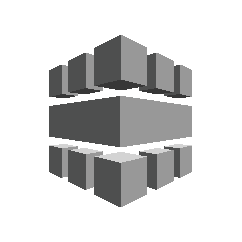
\includegraphics[width=0.9\linewidth]{./pics/aws/ApplicationServices_GRAYSCALE_AmazonElasticTranscoder.eps}
%\end{wrapfigure}



%\paragraph{Cognito}
%\begin{wrapfigure}{i}{0.16\textwidth}
%	
\includegraphics[width=0.9\linewidth]{./pics/aws/MobileServices_GRAYSCALE_AmazonCognito.eps}
%\end{wrapfigure}


%Foo bar ist \lstinline|f = 2 + 2| wasd asdf 

%\section{Technologien}
%Microsoft Azure Funktions 
%AuthO : AuthO
%Firebase : Google
%Stack Driver Logging : Google
%Cloud Machine Learning Engine : Google
%Cloud DataFlow : Google -> Stream batch pipelines
%Big Query : Google




%Befehlmuster wird bei Fusekiserver\ref{komponenten:fuseki} als erteiler der Httpanfrage indem die SparQL Abfrage weiterleiten kann. Daher wird ein Pfad haus/hunde und haus/katze zur gleichen Funktion führen.
%Dieser kann aber offline gehen, also mehreren priorisierten MessagePattern als Queue vor eine oder mehreren Lambdas zu setzen absichert die Stabilität des Systems und entkoppelt Komponenten @RoundRobin?? BSRN.
%Die Verkettung von Funktionen mittels \glqq Pipes\grqq erlaubt die mehrfache Filterung von Daten.

%\section{Guidance}
%Caching -> Lambda Reads Same source and Process
%Compute partitioning -> Lambda per use. solved
%Data Consistency -> Embrace Eventual Consistency in Distributed DBs
%Data partitioning <-> Sharding 
%Instrumentation and Telemetry Guidance -> Errors Handling
%Service Metering -> understand future use of services
